\documentclass[a4paper,10pt]{report}
\usepackage[french]{babel}
\usepackage[utf8]{inputenc}
\usepackage[left=2.5cm,top=2cm,right=2.5cm,nohead,nofoot]{geometry}
\usepackage{url}
\usepackage[T1]{fontenc}
\usepackage{float}
\usepackage{afterpage}
\usepackage{amsmath}
\usepackage{graphicx}
\usepackage{tabularx}
\usepackage{csquotes}
\usepackage{fullpage}

\usepackage[pdftex,
            pdfauthor={A. Caccia, A. Madeira Cortes, N. Marchant, R. Fontaine},
            pdftitle={Contrôle automatique d'une serre},
            pdfsubject={Contrôle automatique d'une serre}]{hyperref}

\linespread{1.1}

\setlength{\parskip}{0.5em}

\begin{document}

\begin{titlepage}
    \begin{center}
        \textbf{\textsc{Université Libre de Bruxelles}}\\
        \textbf{\textsc{Faculté des Sciences}}\\
        \textbf{\textsc{Département d'Informatique}}

        \vfill{}
        \vfill{}

        \begin{center}
            {\Huge Contrôle automatique d'une serre}
        \end{center}

        {\Huge \par}

        \begin{center}
            {\large A. Caccia, A. Madeira Cortes, N. Marchant, R. Fontaine}
        \end{center}

        {\Huge \par}
        \vfill{}
        \vfill{}

        \begin{flushleft}
            {\large \textbf{Superviseurs :} M. Labbé, T. Lenaerts}
            \hfill{}
        \end{flushleft}

        {\large\par}
        \vfill{}
        \vfill{}
        % \enlargethispage{3cm} % do not remove

        \textbf{Année académique 2015--2016}
    \end{center}
\end{titlepage}

\renewcommand{\abstractname}{Abstract}
\begin{abstract}

Le but de ce rapport est d'analyser des algorithmes de contrôle et leurs améliorations possibles, tout comme présenter une implémentation de ceux-ci qui a été faite dans le cadre du Printemps des Sciences de l'Université Libre de Bruxelles (Belgique).

Les algorithmes de contrôle étudiés sont Bang bang, PID (ainsi que ses variantes) et MPC. Suite au choix d'implémenter les deux premiers, les diverses techniques pour améliorer PID on été étudiées et comparées. Ces techniques ont pour but de chercher des paramètres optimaux minimisant une fonction de score. Diverses métriques de score ont été utilisées.

-- RÉSULTATS ICI --

Ces algorithmes ont été implémentés dans une situation réelle, la création d'une serre qui fonctionne en autogestion. Celle-ci utilise les algorithmes de contrôle étudiés pour garder la température, luminosité et humidité du sol proches d'une valeur consigne.


\end{abstract}


\tableofcontents


\chapter{Introduction}

Le but du projet était de créer une serre fonctionnant de façon autonome. Au vu de la pollution grimpant de façon astronomique dans les grandes villes et mégalopoles, de nombreuses méthodes pour baisser les émissions de gaz à effet de serre ont été créées depuis quelques années. L'une d'elles est de construire des serres dans les toits ou caves inutilisées d'immeubles, et de préférence les automatiser.

Cette technique a pour grand avantage, si exploitée de façon efficace, de réduire considérablement le nombre de camions entrant et sortant de la ville pour effectuer des livraisons. De plus, dans certains cas, le rendement est jusqu'à 100 fois plus grand, pour 40\% moins d'énergie consommée, 40\% moins de pertes d'aliments et 99\% moins d'utilisation d'eau que la production traditionnelle. \cite{GEReports}

Pour construire une telle serre il était nécessaire d'étudier en détail le matériel requis pour l'automatiser, notamment les capteurs et mécanismes à créer pour analyser et modifier l'environnement de celle-ci en temps réel.
Ensuite, il était important d'étudier et analyser un type d'algorithmes dits de ``contrôle'', qui nous permettraient de créer l'aspect automatisé de la serre.


\chapter{État de l'art}

Cet état de l'art est séparé en deux parties : la première détaille les différentes méthodes de régulation automatique et la seconde étudie les différentes méthodes pour configurer l'algorithme \emph{PID}, détaillé en \ref{PID}.

\section{Contrôle automatique}
L’automatique est une science qui étudie la modélisation, l’analyse et la commande de systèmes dynamiques.
L’automatique permet de contrôler un système en respectant un cahier des charges (rapidité, précision, stabilité, ...).

L'automatique était un sujet assez vaste, nous nous limiterons ici à l'étude des différentes méthodes de contrôle permettant de stabiliser l'état d'un système au plus proche d'une valeur consigne.

Nous étudierons premièrement \emph{BangBang}, l'algorithme le plus simpliste, utilisé dans les thermostats.
Ensuite nous étudierons \emph{PID} ainsi que ses variantes.
Pour finir nous survolerons \emph{MPC}, un algorithme prédictif plus avancé.

\subsection{\emph{Bang bang}}
Le \emph{``Bang bang control''} aussi appelé \emph{``On-Off control''} ou en français \emph{``Tout ou rien''} est un contrôleur qui ne peut accepter que deux états de contrôle tels que ouvert ou fermé, allumé ou éteint.

Des exemples très classiques d'utilisation de ce type de contrôleur sont les thermostats: le chauffage s'allume sous une température minimale, et s'éteint au-dessus d'un seuil maximal.

Nonobstant la facilité d'implémentation et de mise en place de cet algorithme, son utilisation ne peut être généralisée au contrôle de phénomènes spontanés. En effet, si l'on prend l'exemple du contrôle de la luminosité, \emph{bang bang} ne pourra qu'allumer ou éteindre des lampes, il ne pourra influer sur leur intensité. \cite{Burghes2004}

De plus, cet algorithme ne permet pas une stabilité suffisante : en effet, une fois la correction atteinte, \emph{Bang bang} agira plus jusqu'à ce que les perturbations soient trop importantes et cela produira une oscillation permanente. \cite{ballard1993pid}


\subsection{\emph{PID}}
\label{PID}

\emph{PID} est le régulateur le plus connu et le plus utilisé dans le domaine industriel : il serait utilisé dans plus de 95\% des systèmes \cite{Kinnaert2013, aastrom2002control}.
Il porte ce nom à cause de son fonctionnement qui est découpé en trois actions : l'action proportionnelle, l'action intégrale et l'action dérivée.

PID est défini par la fonction suivante:

\begin{equation}
  u(t) =
    \underbrace{K_p e(t)}_{P} +
    \underbrace{K_i \int_{0}^{t} e(\tau) d\tau}_{I} +
    \underbrace{K_d \frac{de}{dt}.}_{D}
\end{equation}

Dans laquelle $u(t)$ est la sortie de PID qui doit être appliquée à l'élément à contrôler et P, I et D sont les trois composantes ci-dessous :
\begin{description} %TODO: syntaxe, où es-tu ?
\item[Action proportionnelle (P) :]
    est proportionnelle à l'erreur de contrôle courante.
\item[Action intégrale (I) :]
    fait varier la réponse de PID en fonction des valeurs passées de l'erreur de contrôle.
\item[Action dérivée (D) :]
    est basée sur les valeurs futures estimées pour l'erreur de contrôle.
\end{description}

Les premières analyses techniques de \emph{PID} datent de 1922, lorsque Nicolas Minorsky essaye de créer des systèmes de pilotage automatique pour la marine des États-Unis. \cite{minorsky1922directional}

Malgré le fait que de nombreuses autres techniques ont été inventées depuis la création de \emph{PID}, il maintient son fonctionnement de base et a simplement évolué avec le temps et sert parfois de composant de base à d'autres contrôleurs plus complexes \cite{ang2005pid} \cite{visioli2006practical}

Il maintient sa popularité car il est souvent admis qu'aucun autre contrôleur n'égale la simplicité, le fonctionnement clair, la facilité d'application et d'utilisation offerte par \emph{PID}. Cette facilité d'utilisation vient du fait qu'il se base uniquement sur des variables mesurées, sans connaissance du procédé sous-jacent et qu'il a donc énormément d'applications différentes \cite{bennett1993history}.

Il est aussi possible dans quelques applications de PID que certaines actions soient inutiles.
Dans ce cas-là, on parle de contrôleurs PI, PD, P ou I.
Par exemple, une des raisons d'enlever l'action dérivée est qu'elle est fort sensible au bruit lors des mesures \cite{svrcek2014real}.

\subsection{P controller}
Le \emph{Proportional Control} est l'ancêtre du PID, il ne prend en compte que la partie proportionnelle de celui-ci.
Cet algorithme se situe entre l'algorithme Bang Bang et PID:
en effet, là où \emph{Bang Bang} va corriger l'état simplement en allumant ou en éteignant un appareil, l'algorithme P control va lui, appliquer une réponse appropriée à la perturbation.

Un tel contrôleur s'exprime par l'équation
\begin{equation}P_{out} = K_{P}e(t) + p_0\end{equation}
dans laquelle $e(t)$ est l'erreur (la différence entre valeur attendue et valeur mesurée), $K_{P}$ est le paramètre de gain proportionnel, $P_{out}$ est la réponse à la perturbation et $p_0$ est la correction à appliquer, nécessaire vu que cet algorithme n'a pas de composante intégrale (contrairement à PID).

Un grand avantage de l'utilisation de ce type de contrôleur est qu'il n'y a qu'un seul paramètre à configurer, qui définit à quel point la correction sera agressive : plus le paramètre $K_{p}$ est petit (respectivement grand), plus la réaction est lente (respectivement rapide).

Si l'implémentation d'un tel contrôleur est aisée, ses sorties produisent un phénomène d'\emph{offset} : un décalage par rapport aux valeurs attendues \cite{svrcek2014real}.

Le choix d'un tel contrôleur par rapport à PID dépend de l'utilisation, de la précision et de la vitesse des corrections désirées.
Des exemples où l'algorithme P control est suffisant sont donnés dans \cite{sellers2001overview}.

\subsection{\emph{Integral controller}}
Le principe d'un \emph{Integral controller} est de corriger un offset résultant de l'utilisation d'un P controller.
Un tel contrôleur est caractérisé dans \cite{svrcek2014real} par l'équation
\begin{equation}P_{out} = \frac{1}{T_{i}}\int e dt + MV_{0}\end{equation}
où $MV_{0}$ correspond à la correction biaisée de P controller,
$\int e dt$ représente l'intégrale des erreurs sur l'intervalle de temps $dt$ et $T_{i}$ est le temps intégral défini comme le temps nécessaire pour changer la sortie du contrôleur d'une quantité égale à l'erreur.

Bien que ce contrôleur propose une correction aux décalages, on observe un temps de réponse jusqu'à dix inférieur inférieur à l'utilisation d'un P controller seul \cite{svrcek2014real}.

\subsection{PI controller}
Un contrôleur PI utilise à la fois l'action proportionnelle et l'action intégrale.
Il est caractérisé par l'équation
\begin{equation}P_{out} = K_{P} e + K_{I} \int e dt\end{equation}
où $K_{p}$ et $K_{I}$ sont les paramètres de réglages proportionnel et intégral
et les autres symboles correspondent à ce qui est indiqué dans les sections \emph{P controller} et \emph{Integral controller}.

Ces contrôleurs sont 50\% plus lents qu'un contrôleur P seul, mais plus rapides que l'ajout d'un contrôleur intégral séparé \cite{svrcek2014real}.
En effet, si l'on compare son équation avec celle du P controller, le terme $p_0$ a été remplacé par une correction intégrale, ce qui corrige l'erreur automatiquement.

\subsection{MPC controller}
\emph{MPC} est un contrôleur permettant la régulation de différentes variables dans un système.
Celui-ci utilise à la fois des stratégies prédictives et l'état actuel afin de calculer les prochaines états possibles \cite{RICHALET1978413}.

Contrairement à PID, MPC accepte des systèmes ayant de multiples valeurs d'entrées et devant sortir également plusieurs valeurs.
Par contre, de nombreux modèles MPC ne supportent que les circuits en boucle ouverte.
Il demande également plus de ressources à la fois logicielles et matérielles \cite{saletovic2014apm}.
De plus, ils nécessitent un grand nombre de modèles pour interpoler la réponse et si la commande prédictive est erronée, les performances vont être faibles même si les modèles sont corrects \cite{Richalet2016}.

Une comparaison entre APM (une variante simple de MPC) et PID a été faite dans \cite{saletovic2014apm}, et montre qu'avec des configurations optimales, APM a apporté un meilleur contrôle que PID, mais PID a requis moins de ressources et possède un temps de stabilisation plus court.

\section{Détermination des paramètres de PID}

\emph{PID} étant inefficace et donc inutile si ses paramètres (les constantes $K_p$, $K_i$, $K_d$) sont mal fixés, il nous semble important d'aussi étudier les différentes méthodes pour les déterminer. Il existe énormément de méthodes différentes pour configurer \emph{PID}.

Nous étudierons ici trois méthodes manuelles ainsi que deux méthodes heuristiques.

Nous encourageons le lecteur à se référer à \cite{shahrokhi2013comparison} qui fait une revue plus détaillée et complète des différentes méthodes pour déterminer les paramètres.


\subsection{La méthode manuelle}

La méthode manuelle est une technique où un opérateur humain modifie les paramètres manuellement, sans algorithme déterminé, jusqu'à obtenir un résultat satisfaisant. Cette technique s'applique sur un système en fonctionnement.

L'avantage de cette technique est qu'elle ne nécessite aucun calcul mathématique complexe. Cependant, elle requiert l'interaction d'un technicien expérimenté, étant donné que chaque variation des paramètres implique de très nombreuses modifications sur le résultat obtenu (croissance initiale, stabilité, délai d'attente jusqu'à la stabilité, dépassement, ...). \cite{zhong2006pid}


\subsection{Ziegler–Nichols}
% ziegler1942optimum
% silva2007pid
% http://www.chem.mtu.edu/~tbco/cm416/tuning_methods.pdf
Comme la méthode manuelle, Ziegler–Nichols s'applique aussi sur un système en fonctionnement. Cependant, elle utilise des calculs un peu plus complexes que la méthode manuelle mais son avantage est qu'elle nécessite des techniciens moins expérimentés.\cite{ziegler1942optimum}
En effet, cette méthode requiert peu d'informations sur le système en fonctionnement, étant donné que les formules utilisées découlent d'un nombre exhaustif de simulations de systèmes stables et simples. \cite{silva2007pid}

Une des critiques qui peut être faite à cette méthode est que dans la plupart du temps elle donne des bons résultats mais dans certains cas le résultat est fort erroné,
menant à un mauvaise stabilité et un faible amortissement des perturbations.

De plus, cette méthode produit systématiquement un dépassement lors de la montée initiale et
puis se met à osciller avec une amplitude d'oscillation qui décroit linéairement au cours du temps.
Elle n'est donc pas utilisable dans tout les système
 et est particulièrement déconseillée lorsque le système ne peut pas dépasser fortement la valeur cible \cite{silva2007pid}.

\subsection{Recherche Tabou}

Il est aussi possible de déterminer des paramètres pour PID à l'aide la méthode de la recherche Tabou.

La recherche Tabou est une méthode heuristique d'optimisation utilisée quand l'expression analytique de la fonction à minimiser n'est pas connue
(comme dans le cas de PID si le système à stabiliser n'a pas été modélisé mathématiquement ou physiquement).

La recherche Tabou est une recherche locale qui part d'un point arbitraire et compare ses points proches afin de tenter de trouver le minima de celle-ci.
Le mot Tabou vient du fait qu'il faut pas tomber dans un minima local et y rester :
cet algorithme garde donc une liste des minimas locaux, la liste des tabous, pour ne pas y retomber.

Une comparaison entre résultats obtenus avec la méthode de Ziegler-Nichols et la recherche Tabou se trouve dans \cite{Karaboga569754}.
Une autre implémentation citée dans \cite{bagis2011tabu} compare la recherche Tabou avec plusieurs autres algorithmes et démontre l'efficacité de la méthode.

\subsection{Algorithme génétique}

Les algorithmes génétiques sont un type d'algorithme évolutif qui mimique la théorie de l'évolution afin de rafiner des résultats par un procédé iteratif aléatoire, ce qui en fait une méthode métaheuristique.

Plusieurs avantages et inconvénients sont discutés dans \cite{Tabassum2014}.
Par exemples, ces algorithmes permettent l'optimisation d'une large variété de problèmes et sont efficaces pour déterminer plusieurs paramètres à la fois.
Cependant, ces algorithmes nécessite une grande taille de population et beaucoup de générations pour converger vers un bon résultat, ce qui peut tendre vers des temps d'exécutions assez élevés.
De plus, un mauvais choix de la fonction de score (\ref{section:metrics}) pourra conduire à un résultat exécrable qui ne sera remarqué qu'à la fin de l'exécution de l'algorithme.

Une comparaison des performances obtenues entre un PID paramétré via la méthode de Ziegler-Nichols et via un algorithme génétique et a montré un temps de réponse beaucoup plus rapide avec cet algorithme dans \cite{thomas2009position}.

\chapter{Méthodes implémentées}
\label{chap:impl}

Nous avons décidé d'implémenter \textit{Bang-bang} et \textit{PID} ainsi que différentes méthodes pour déterminer les paramètres de \textit{PID} afin de pouvoir les comparer par la suite.

%TODO être sérieux
Ces implémentations ont été réalisées dans le langage de programmation Python, afin de tirer parti de sa rapidité de développement et ses librairies de calcul scientifique, telles que Numpy et Scipy.

\section{Contrôle automatique}
\label{sec:contr-implem}
Le contrôle automatique étant dominé par la combinaison de \textit{Bang-bang} et \textit{PID}, nous avons choisi d'étudier en détail ces deux-ci ainsi que les variantes \textit{P} et \textit{PI}.

\subsection{\emph{Bang-bang}}

L'implémentation de \emph{Bang-bang} est simple: une fonction reçoit en paramètre la variable à contrôler et observe si celle-ci est en-dessous (respectivement au-dessus) d'un seuil dans le cas où la correction tend à augmenter (respectivement diminuer) la variable. Elle renvoie ensuite en conséquence un état: allumé ou éteint.

L'implémentation que nous avons écrite fonctionne simplement : à chaque fois que la fonction de contrôle est appelée, elle regarde si l'entrée est trop basse et si oui, la sortie est l'état activé, si non, l'état désactivé.

\subsection{PID}

\emph{PID} tentant de minimiser l'erreur au long du temps en s'ajustant peu à peu, son implémentation est un peu plus complexe : à chaque appel à la fonction de contrôle, l'erreur courante ainsi que le temps sont enregistrés.
Il est ensuite possible de calculer l'intégrale des erreurs du passé ainsi que la dérivé de l'erreur à l'instant présent.
Nous pouvons donc utiliser ces différentes valeurs pour les introduire dans la formule de PID et les pondérer à l'aide des paramètres ($K_p$, $K_i$ et $K_d$) qui ont été spécifiés pour l'instance du contrôleur et la sortie de cette formule nous donnera la correction à appliquer.

De plus, quand la correction à appliquer dépasse la valeur maximale de que le composant physique peut accepter (par exemple, on ne peut demander à une ampoule allumée à fond de briller plus), pour éviter qu'une erreur qui n'est pas complètement corrigeable à cause de limitations physiques ne pénalise trop la partie intégrale dans le futur, nous tronquons la valeur ajoutée à cette intégrale à la limite physique.

\section{Détermination des paramètres de PID} %TODO: refactor intro et bouger ceci dans l'état
Les effets (positifs ou négatifs) de l'ajustement des paramètres sont, entre autres \cite{zhong2006pid} :
\begin{enumerate}
\item la stabilité,
\item la précision (l'erreur même quand l'équilibre est atteint),
\item la rapidité (le temps d'attente avant que le système n'arrive à la stabilité)
\end{enumerate}

\subsection{La méthode manuelle}

L'algorithme se déroule en 4 étapes:
\begin{enumerate}
    \item Les valeurs des 3 paramètres sont fixées à $0$.
    \item Le paramètre $K_p$ est incrémenté jusqu'à ce que la sortie du système se mette à osciller.
    On prendra comme valeur pour $K_p$ la moitié de celle obtenue précédemment.
    \item $K_i$ est augmenté jusqu'au moment où l'offset est corrigé dans un temps acceptable pour le système.
    \item Si nécessaire, $K_d$ est augmenté jusqu'au moment où la boucle est suffisamment rapide pour atteindre à nouveau la consigne après une perturbation extérieure.
\end{enumerate}

\subsection{Ziegler–Nichols}

Elle débute comme la méthode manuelle :
\begin{enumerate}
    \item Les valeurs des 3 paramètres sont fixées à $0$.
    \item $K_p$ est augmenté jusqu'à ce que la sortie de la boucle oscille (comme précédemment).
\end{enumerate}

Par contre, cette fois-ci, on va nommer la valeur de $K_p$ ainsi obtenue $K_u$ et la période de l'oscillation $P_u$.
Ensuite, les autres paramètres sont déterminés à l'aide du tableau \ref{tab:ZieglerNicholsTuningFormulas}

\def\tabularxcolumn#1{m{#1}}
\begin{figure}[ht]
    \begin{center}
        \begin{tabularx}{\textwidth}{| c | X | X | X |}
            \hline
            & $K_p$ & $K_i$ & $K_d$\\ \hline
            P & \begin{equation*}\frac{K_u}{2}\end{equation*} & &\\ \hline
            PI & \begin{equation*}\frac{K_u}{2,2}\end{equation*} & \begin{equation*}1,2 \cdot \frac{K_p}{P_u}\end{equation*} &\\ \hline
            PID & \begin{equation*}\frac{K_u}{1,7}\end{equation*} & \begin{equation*}2 \cdot \frac{K_p}{P_u}\end{equation*} & \begin{equation*}K_p \cdot \frac{P_u}{8}\end{equation*} \\
            \hline
        \end{tabularx}
    \end{center}
    \caption{Tableau des formules pour Ziegler–Nichols}
    \label{tab:ZieglerNicholsTuningFormulas}
\end{figure}

\subsection{Recherche Tabou}

Une autre manière utilisée pour déterminer ces paramètres est d'utiliser la recherche tabou. Le but de cette méta-heuristique itérative est de trouver des minimums locaux pour une fonction objectif.

Pour se faire, nous appliquons l'algorithme suivant:
\begin{enumerate}
    \item prendre un point au hasard comme solution,
    \item Évaluer les points voisins,
    \item Choisir le meilleur point admissible parmi ces voisins n'étant pas dans la tabou liste,
    \item Si le le meilleur point admissible est meilleur que notre solution, on remplace notre solution par ce nouveau point,
    \item Nous l'ajoutons à notre liste tabou,
    \item Nous retournons en 2 tant que nous ne rencontrons pas notre condition d'arrêt.
\end{enumerate}

Des conditions d'arrêts sont par exemple une limite de temps ou lorsque la différence de score entre deux solutions est inférieure à un certain palier. \cite{glover2007principles}
\cite{bagis2011tabu}


\subsection{Algorithmes génétiques}
Il est également possible de déterminer ces paramètres à l'aide de ce que l'on appelle ``un algorithme génétique''.
Le principe est de générer une population de chromosomes, des êtres virtuels qui possèdent tous ici 3 emplacements, représentant chacun l'un des paramètres $K_p$, $K_i$ ou $K_d$ à déterminer.

Chaque chromosome sera alors testé: un algorithme PID sera exécuté par chromosome en spécifiant les paramètres de celui-ci, et recevra ensuite un score indiquant ses performances (voir \ref{section:metrics}).

En fonction de ce score, les chromosomes vont être choisis avec plus ou moins de chance, et procréer: une nouvelle génération va être créée qui contiendra le même nombre de chromosome que la précédente. Pour ce faire:
\begin{enumerate}
  \item on choisit deux chromosomes selon une ``roulette wheel selection'': les chromosomes sont choisis aléatoirement, mais avec des probabilités plus importantes selon la grandeur de leur score;
  \item ils vont se reproduire avec un possible ``crossing-over'': il y aura une probabilité faible que les paramètres des deux chromosomes soient choisis chez l'un ou l'autre pour être attribué au chromosome ``enfant'', sinon, l'enfant héritera des trois paramètres de son premier parent;
  \item le chromosome enfant aura ensuite une faible probabilité de subir une ``mutation'': l'un de ses trois paramètres sera changé aléatoirement.
\end{enumerate}

La nouvelle population créée va recommencer le cycle précédent et régénérer une autre population, et ainsi de suite un certain nombre de fois.

À la fin de toutes ces itérations, le meilleur dernier chromosome sera sélectionné en fonction de son score, et ses paramètres seront utilisés par PID.


\chapter{Résultats expérimentaux}

Après avoir implémenté les algorithmes présentés ci-dessus, nous les avons comparés grâce à un dispositif expérimental que nous avons créé.

\section{Méthode expérimentale}
\label{sec:methode}
Nous avons fabriqué une boite opaque dans laquelle se trouve un capteur de lumière ainsi que deux LEDs de puissance. Le capteur ainsi que la première LED sont reliés à un Arduino\footnote{Un Arduino est un micro-contrôleur programmable en c++ est qui peut communiquer avec un ordinateur par une liaison série} qui fait suivre la valeur du capteur à un programme Python que nous avons écrit et qui récupère la valeur de sortie de ce programme pour contrôler la puissance de la LED.

La seconde LED est utilisée pour perturber le système et ainsi pouvoir mesurer la résistance aux perturbations de nos algorithmes.

Pour comparer deux techniques entre elles, nous lançons plusieurs simulations à la suite l'une de l'autre pour chacune d'elles. % TODO : define plusieurs
Et nous attribuons un score à chaque simulation selon les métriques définies en \ref{section:metrics} et le score final d'une méthode est défini comme la moyenne des scores des différentes simulations.

Une simulation consiste en :
\begin{itemize}
    \item Le système est remis à zéro : toutes les lampes sont éteintes et le capteur indique 0 lux.
    \item L'algorithme de contrôle est lancé avec comme consigne de stabiliser le système à 500 lux.
    \item Après 10 secondes, la seconde LED est allumée pour perturber le système
    \item 10 secondes après l'allumage de la seconde LED, la simulation est arrêtée.
    \item Un score est assigné à la simulation en fonction de sa performance.
\end{itemize}

\subsection{Métriques de score}
\label{section:metrics}
Pour nous permettre de comparer les différentes méthodes, nous devons introduire des métriques permettant d'attribuer un score à ces méthodes.
Nous utiliserons ici les métriques utilisées par \cite{griffin2003line, mirzal2012pid} :
\begin{description}
    \item[MSE] : La moyenne de l'erreur au carré (Mean of the Squared Error)
    \item[ITAE] : L'intégrale du temps multipliée par la valeur absolue de l'erreur  (Integral of Time multiplied by Absolute Error)
    \item[IAE] : L'intégrale de la valeur absolue de la magnitude de l'erreur (Integral of Absolute Magnitude of the Error)
    \item[ISE] : L'intégrale de l'erreur au carré (Integral of the Squared Error)
    \item[ITSE] : L'intégrale du temps multipliée par l'erreur au carré (Integral of Time multiplied by the Squared Error)
\end{description}

$$
\textbf{MSE} = \frac{1}{T} \int_0^T e(t)^2 dt,
\textbf{ITAE} = \int t \cdot |e(t)| dt,
\textbf{IAE} = \int |e(t)| dt,
\textbf{ISE} = \int e(t)^2 dt,
\textbf{ITSE} = \int t \cdot e(t)^2 dt
$$


\section{Résultats}

\subsection{Comparaison des métriques de score}

Pour commencer, nous avons comparé les différentes fonctions de score afin de choisir avec laquelle nous allions comparer nos différents résultats. Pour cela, nous avons exécuté 111 simulations de l'algorithme P avec des valeurs de $K_p$ variant entre 0.005 et 0.2.

Nous avons ensuite comparé 2 à 2 chaque métrique de score et nous avons calculé le \textit{rho} de Spearman, pour chaque paire.

% TODO bouger ça dans les méthodes expé ?

Il est ressorti de cette expérience (comme on peut le voir dans la figure \ref{fig:correlation}) que toutes les métriques des scores ont une corrélation de rang assez élevée :
les métriques \textbf{ISE} et \textbf{MSE} étant identiques à un facteur près, il est logique que leur corrélation de rang soit parfaite.
Ensuite, on remarque que les métriques \textbf{ITSE} et \textbf{ITAE} sont aussi fortement corrélées ce qui confirme que ces deux métriques qui prennent en compte le temps en plus de l'erreur sont fort semblables pour cette raison là.

Toutes les métriques ordonnant chaque simulation presque dans le même ordre,
nous avons choisi pour la suite des expériences la plus simple à calculer et à comprendre :
\textbf{MSE}, la moyenne des carrés des erreurs.

\begin{figure}[hb!]
   \centering
   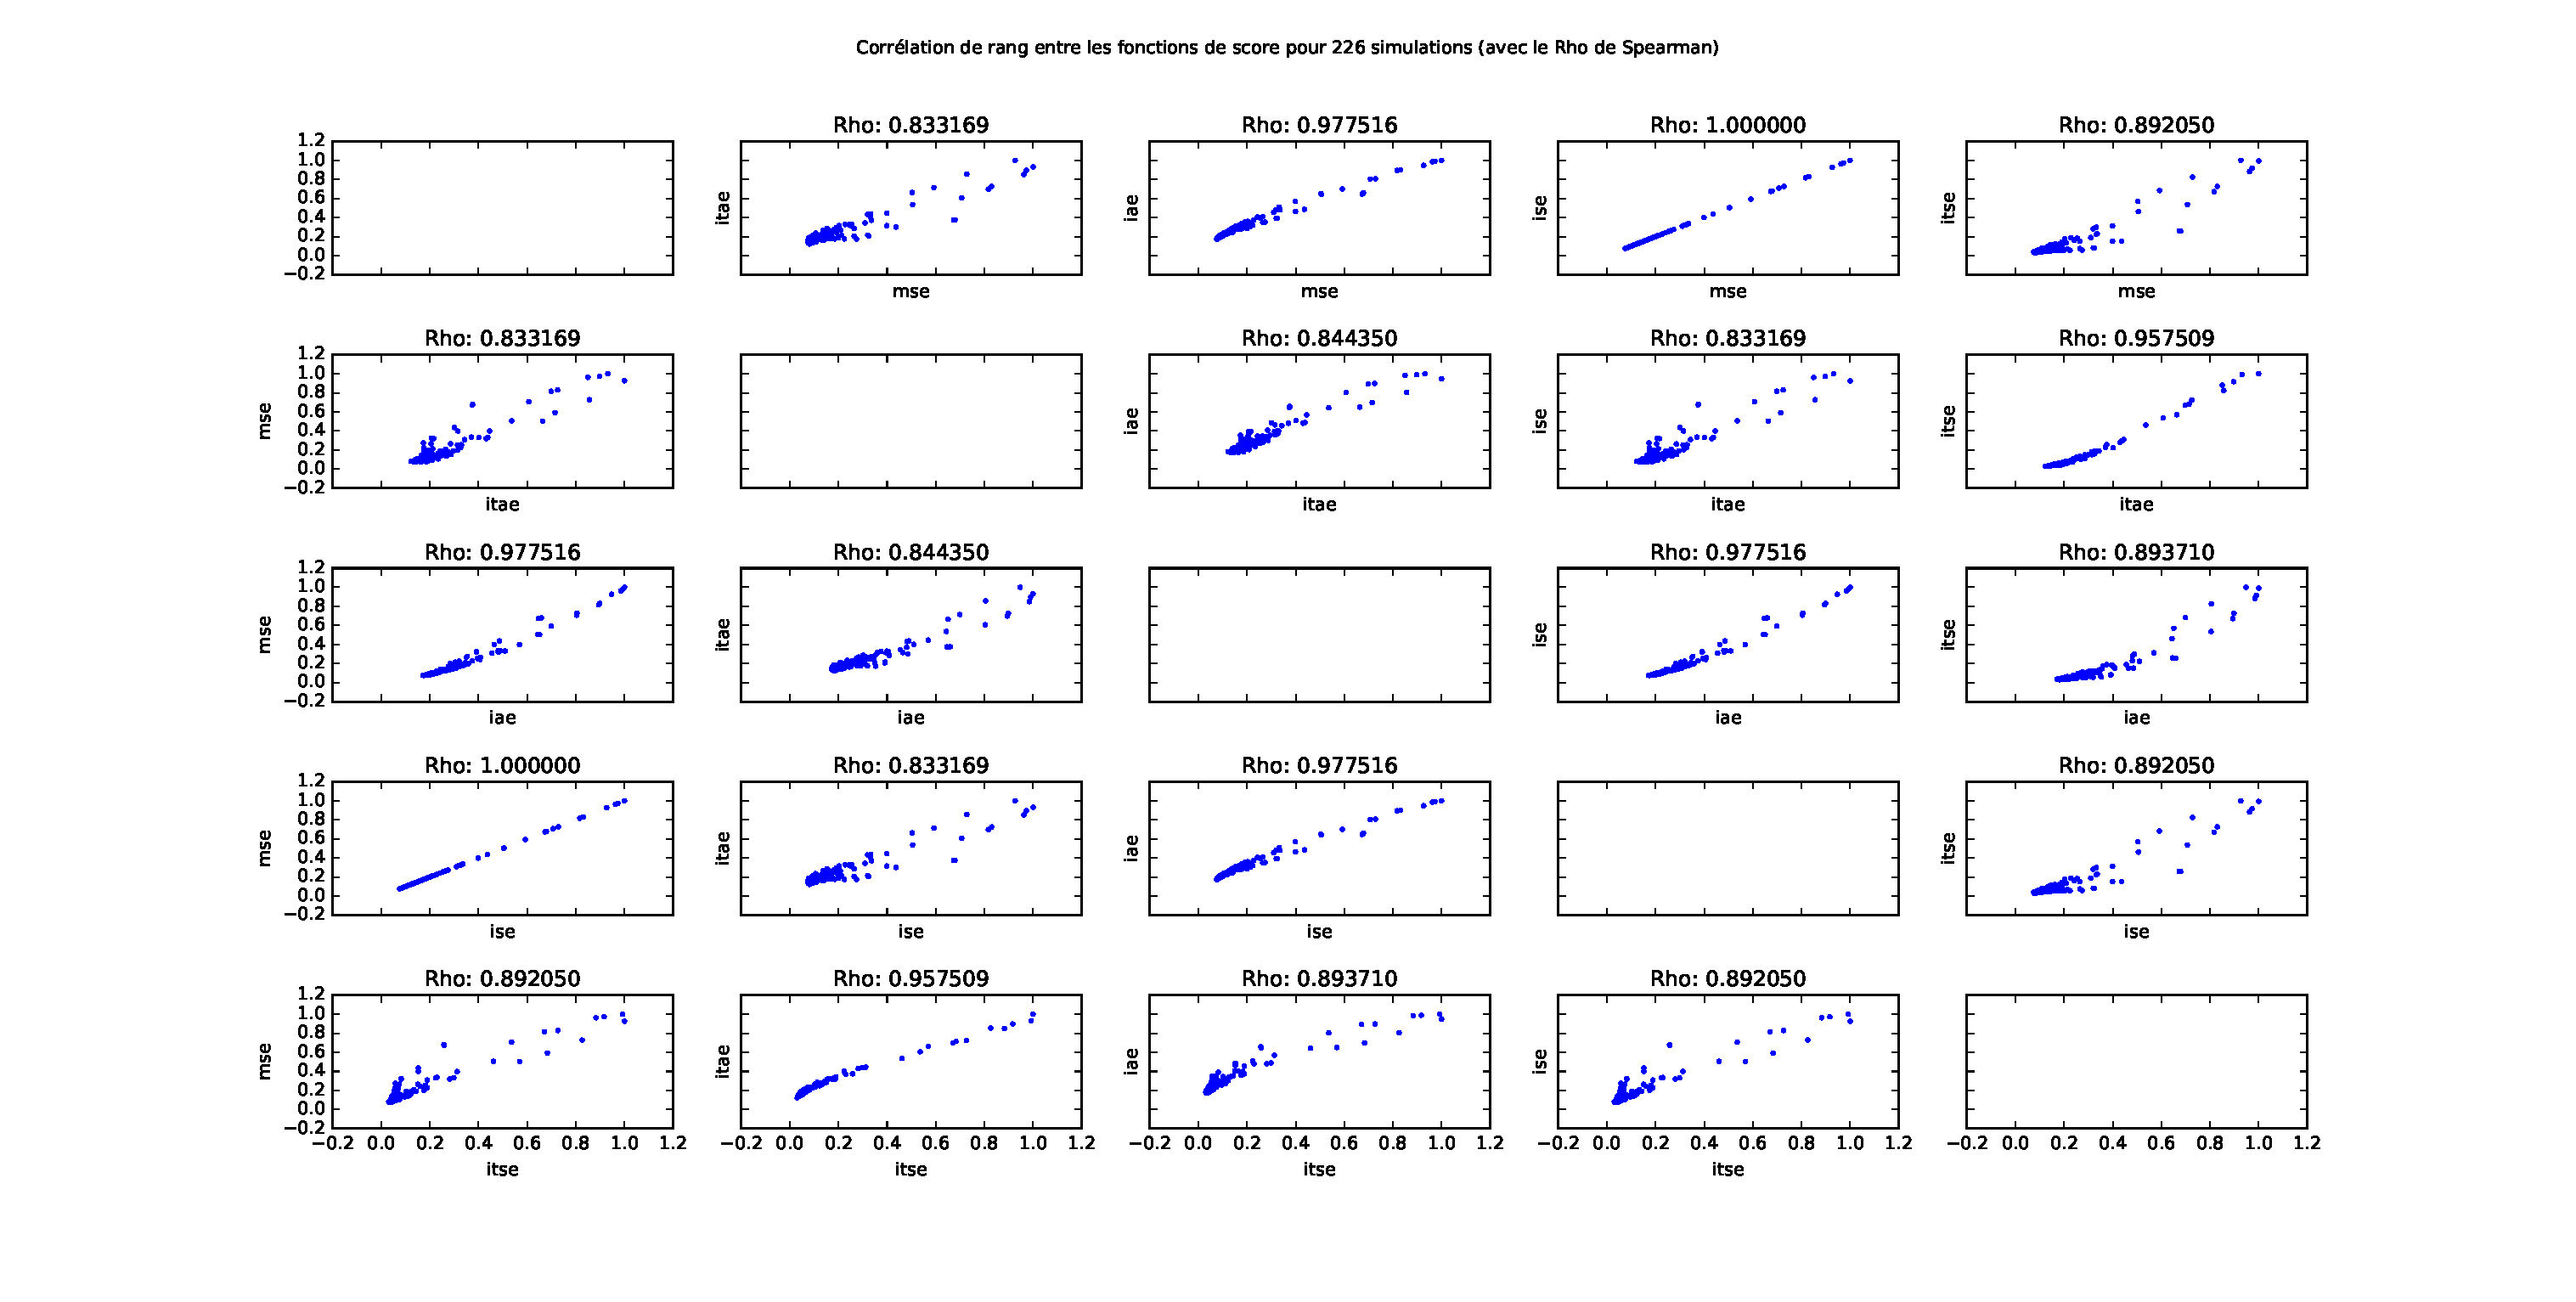
\includegraphics[scale=0.35]{correlation.eps}
   \caption{\label{fig:correlation} Corrélation de rang entre les différentes fonctions de score}
\end{figure}

\subsection{Comparaison des méthodes de contrôle}

Ensuite nous avons comparé les différentes méthodes de contrôle décrites dans la section \ref{sec:contr-implem} ainsi que les variantes \textit{P} et \textit{PI} avec le protocole expérimental décrit dans la section \ref{sec:methode}.

La première constatation est qu'en effet, le fait que \textit{Bang-bang} ne puisse avoir un état allumé ou éteint n'est pas du tout adapté pour réguler un phénomène avec si peu de rémanence comme la lumière.

\subsection{Comparaison des méthodes d'optimisation des paramètres}

Résultats pour chaque méthode

pour genetic : comparer en fct du nombre de générations (et le de taille de la pop)
pour tabu, discuter du nombre de tours à faire avant l'arrêt

\subsection{Comparaison BangBang et P/PI/PID}
Methode de tuning utilisée: Ziegler Nichols
\begin{table}[h]
    \begin{center}
        \begin{tabular}{r l}
            BANG BANG & 548741.789524\\
            P & 45025.847078\\
            PI & 47964.221429\\
            PID & 40209.886443
        \end{tabular}
    \end{center}
    \caption{Score des différents algorithmes de contrôle (moyenne sur 5 simulations)}
\end{table}

\subsubsection{BangBang}
\begin{figure}[hb!]
   \centering
   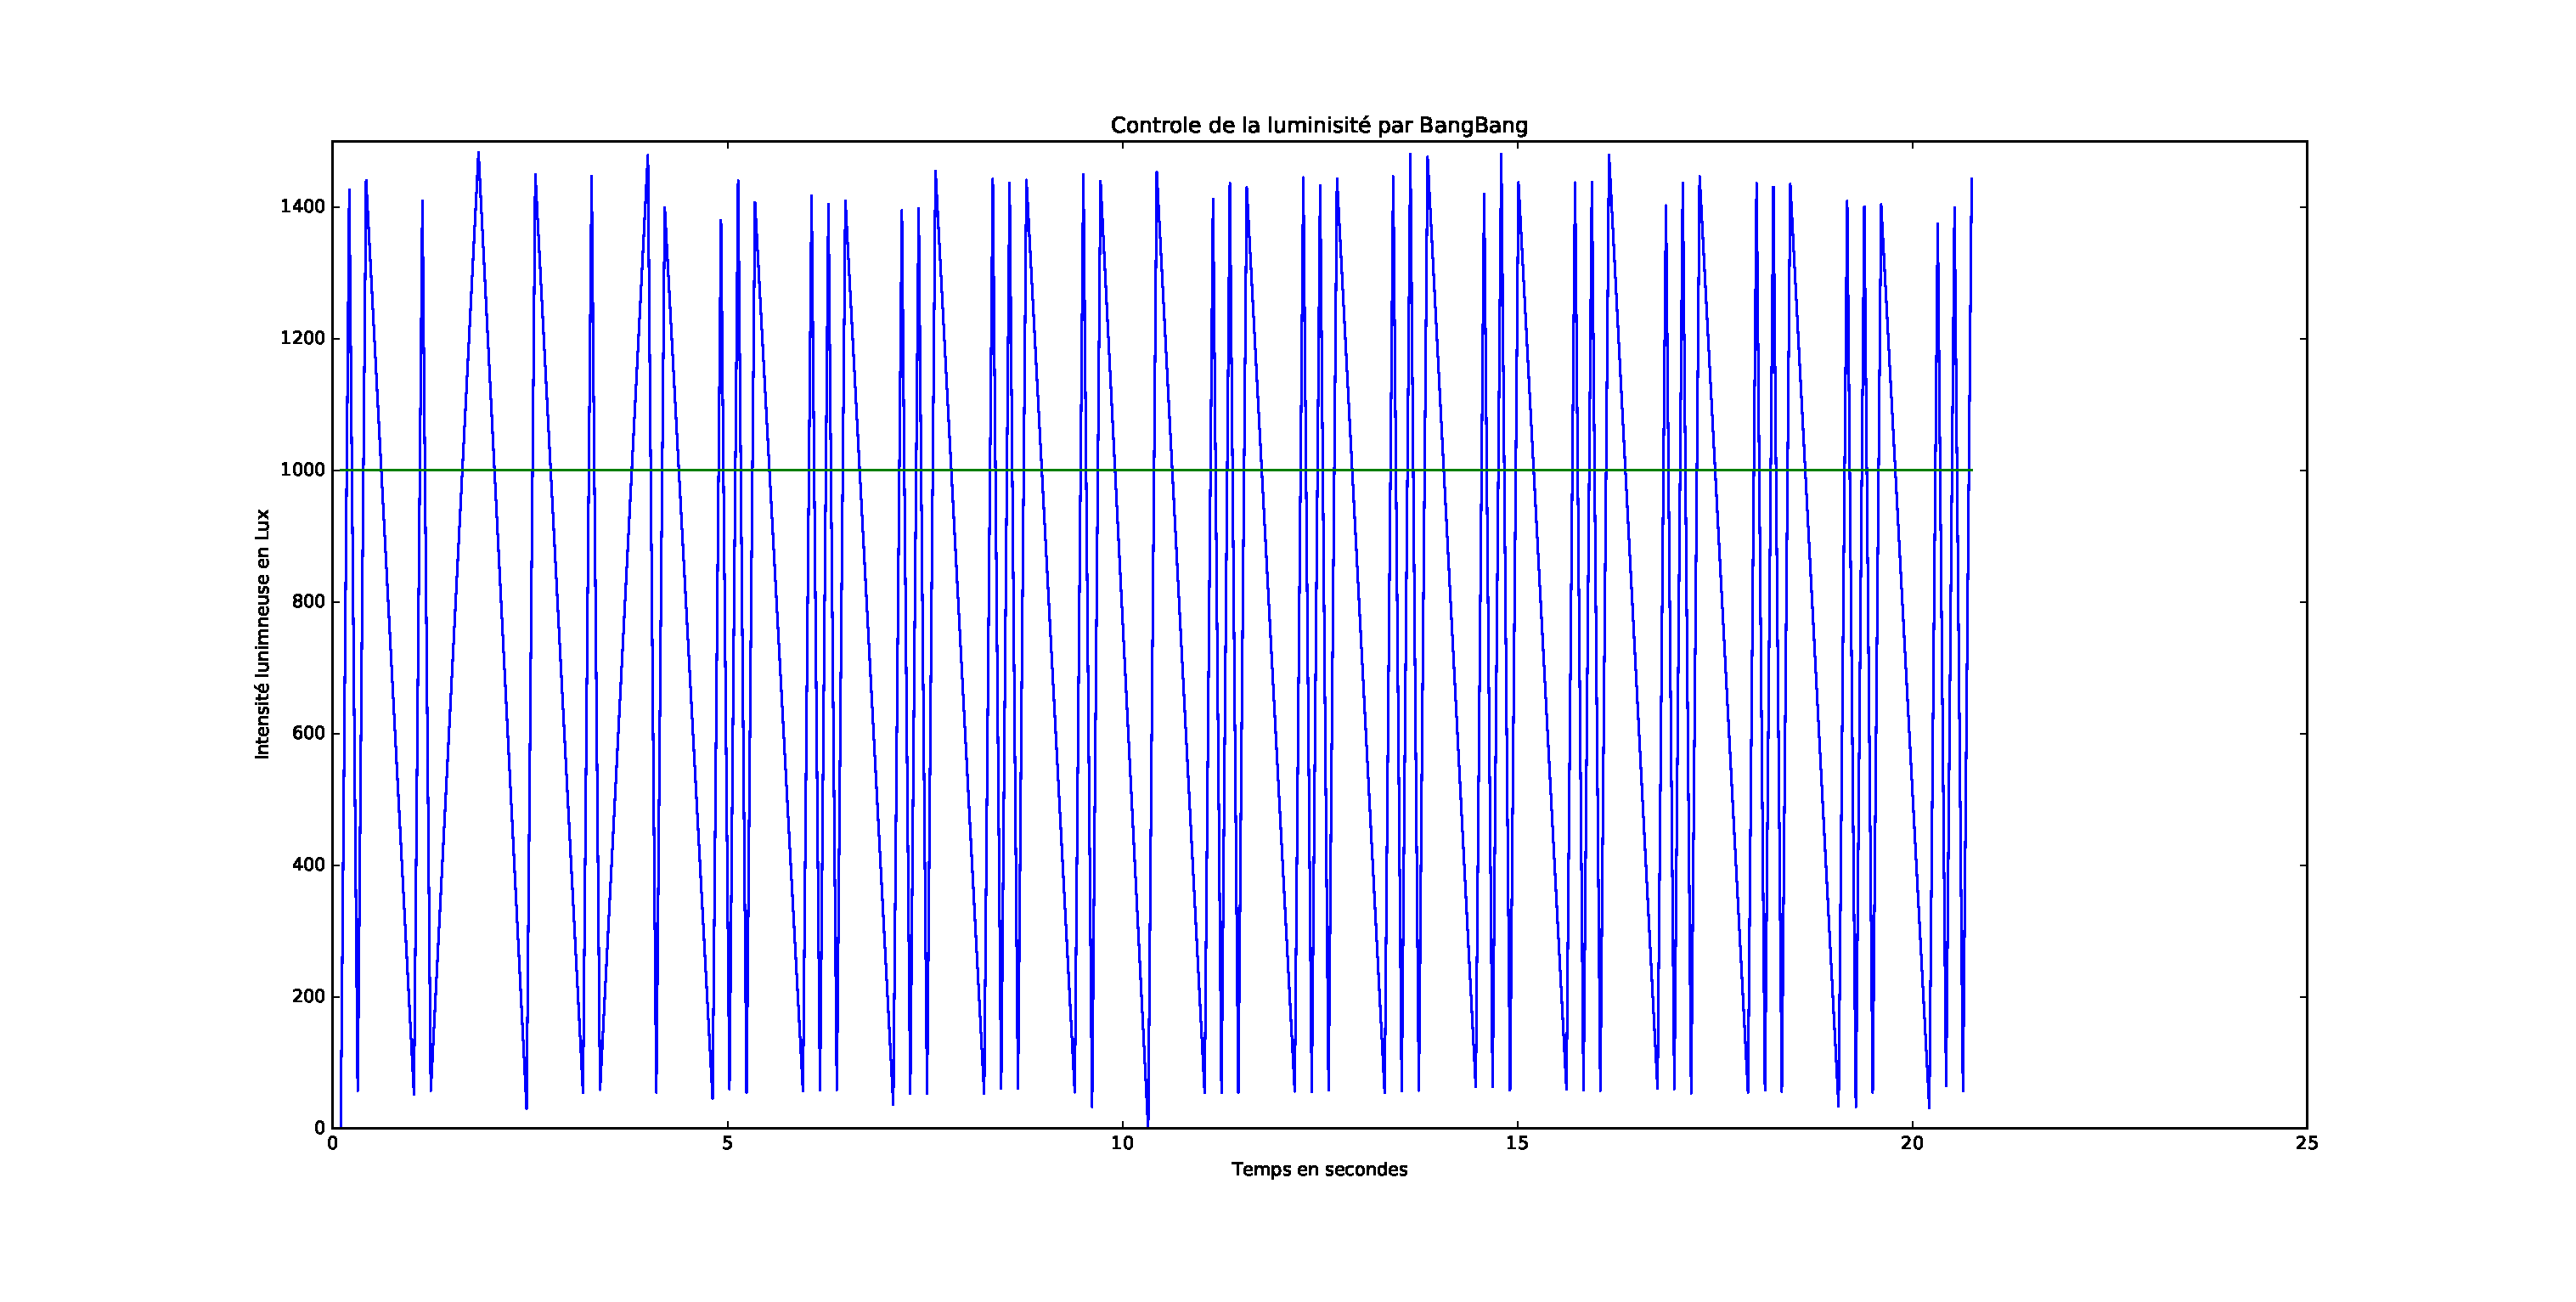
\includegraphics[scale=0.35]{BangBang.eps}
   \caption{\label{fig:bangbang} Contrôle de la luminosité par BangBang}
\end{figure}

\subsubsection{P}
\begin{figure}[hb!]
   \centering
   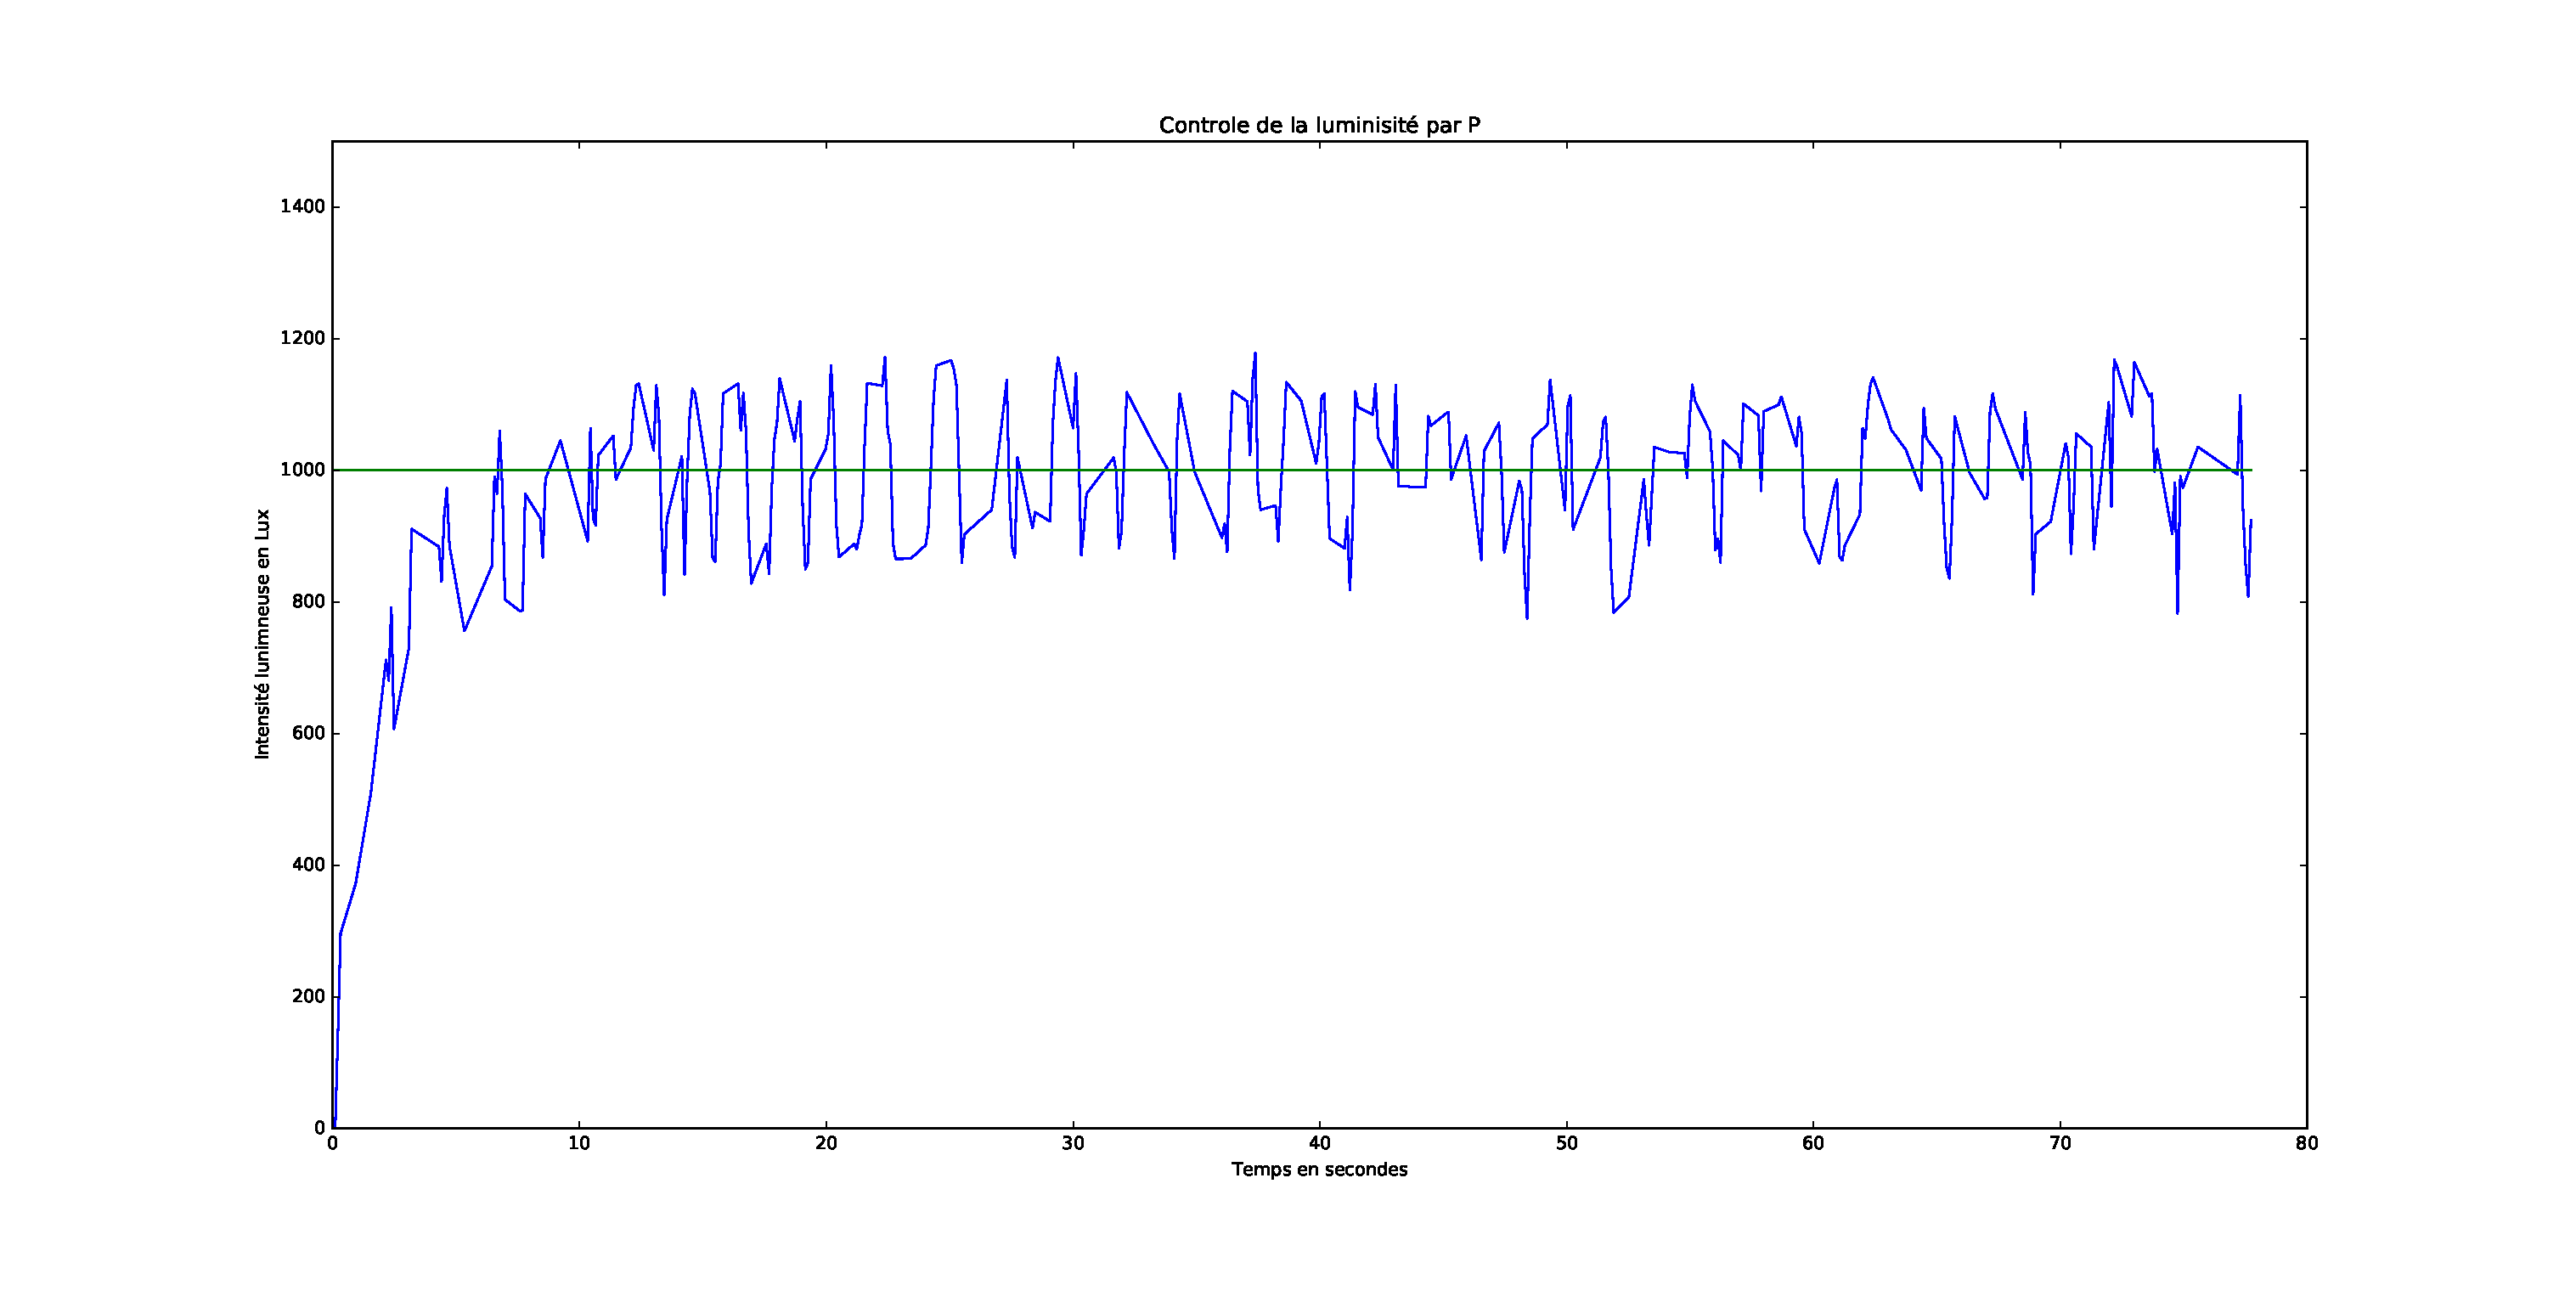
\includegraphics[scale=0.35]{P.eps}
   \caption{\label{fig:p} Contrôle de la luminosité par P}
\end{figure}
Forte oscillation

\subsubsection{PI}
\begin{figure}[hb!]
   \centering
   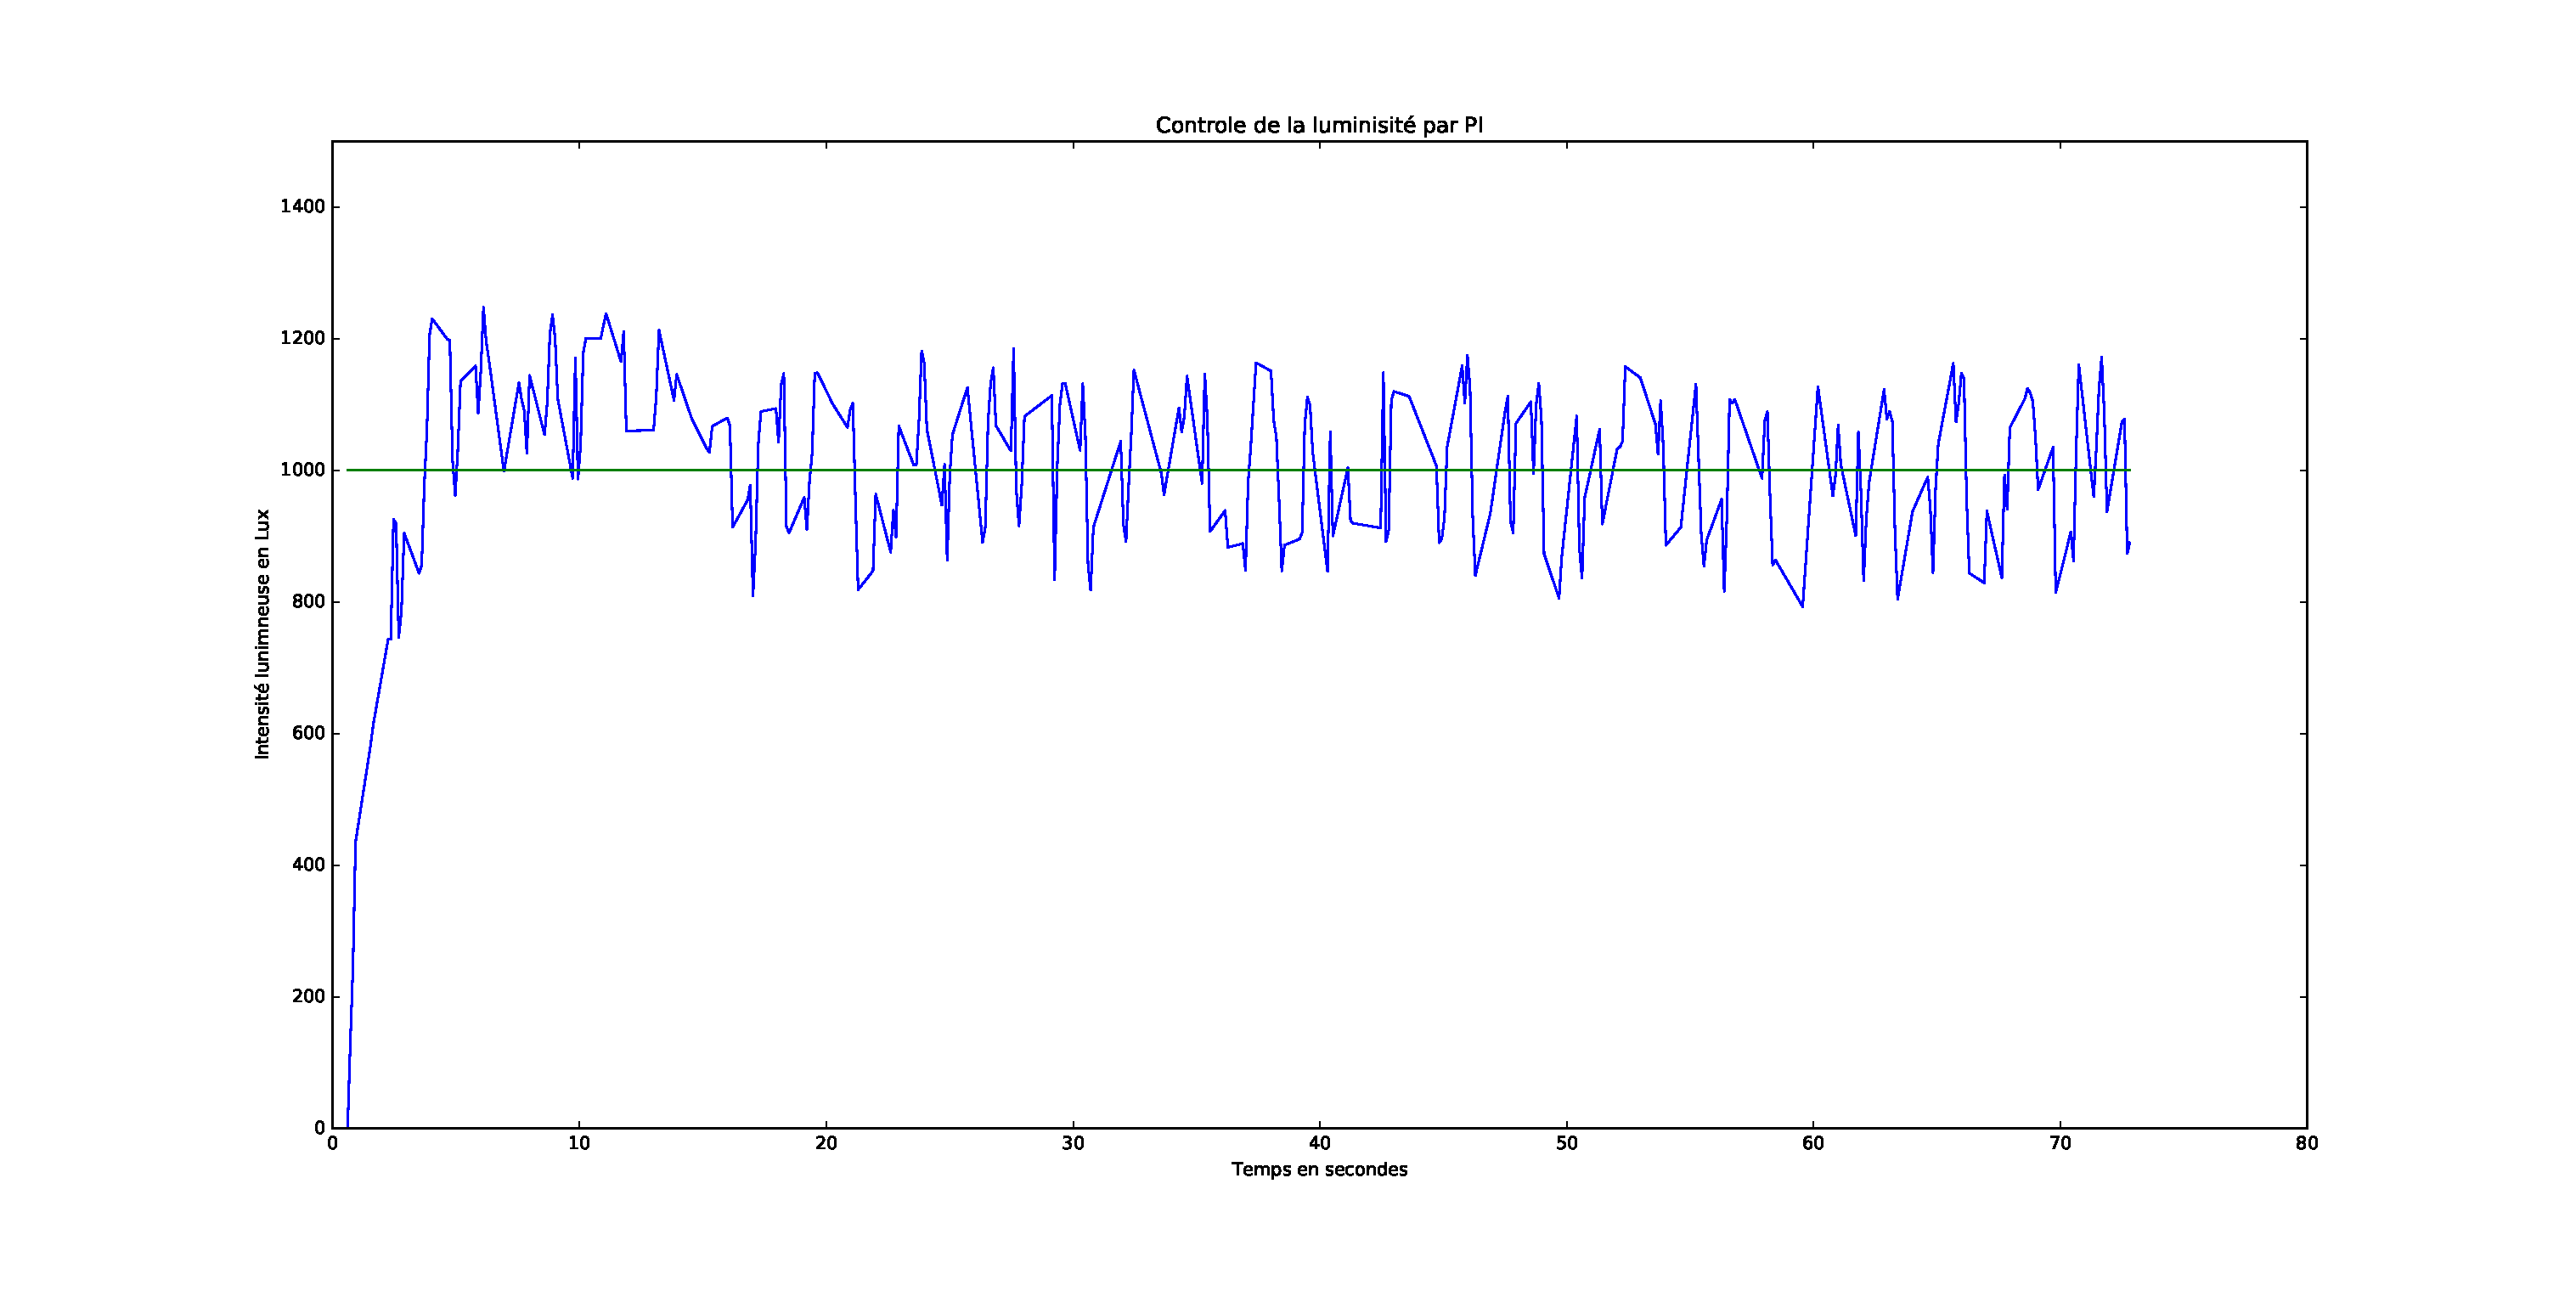
\includegraphics[scale=0.35]{PI.eps}
   \caption{\label{fig:pi} Contrôle de la luminosité par PI}
\end{figure}
Offset

\subsubsection{PID}
\begin{figure}[hb!]
   \centering
   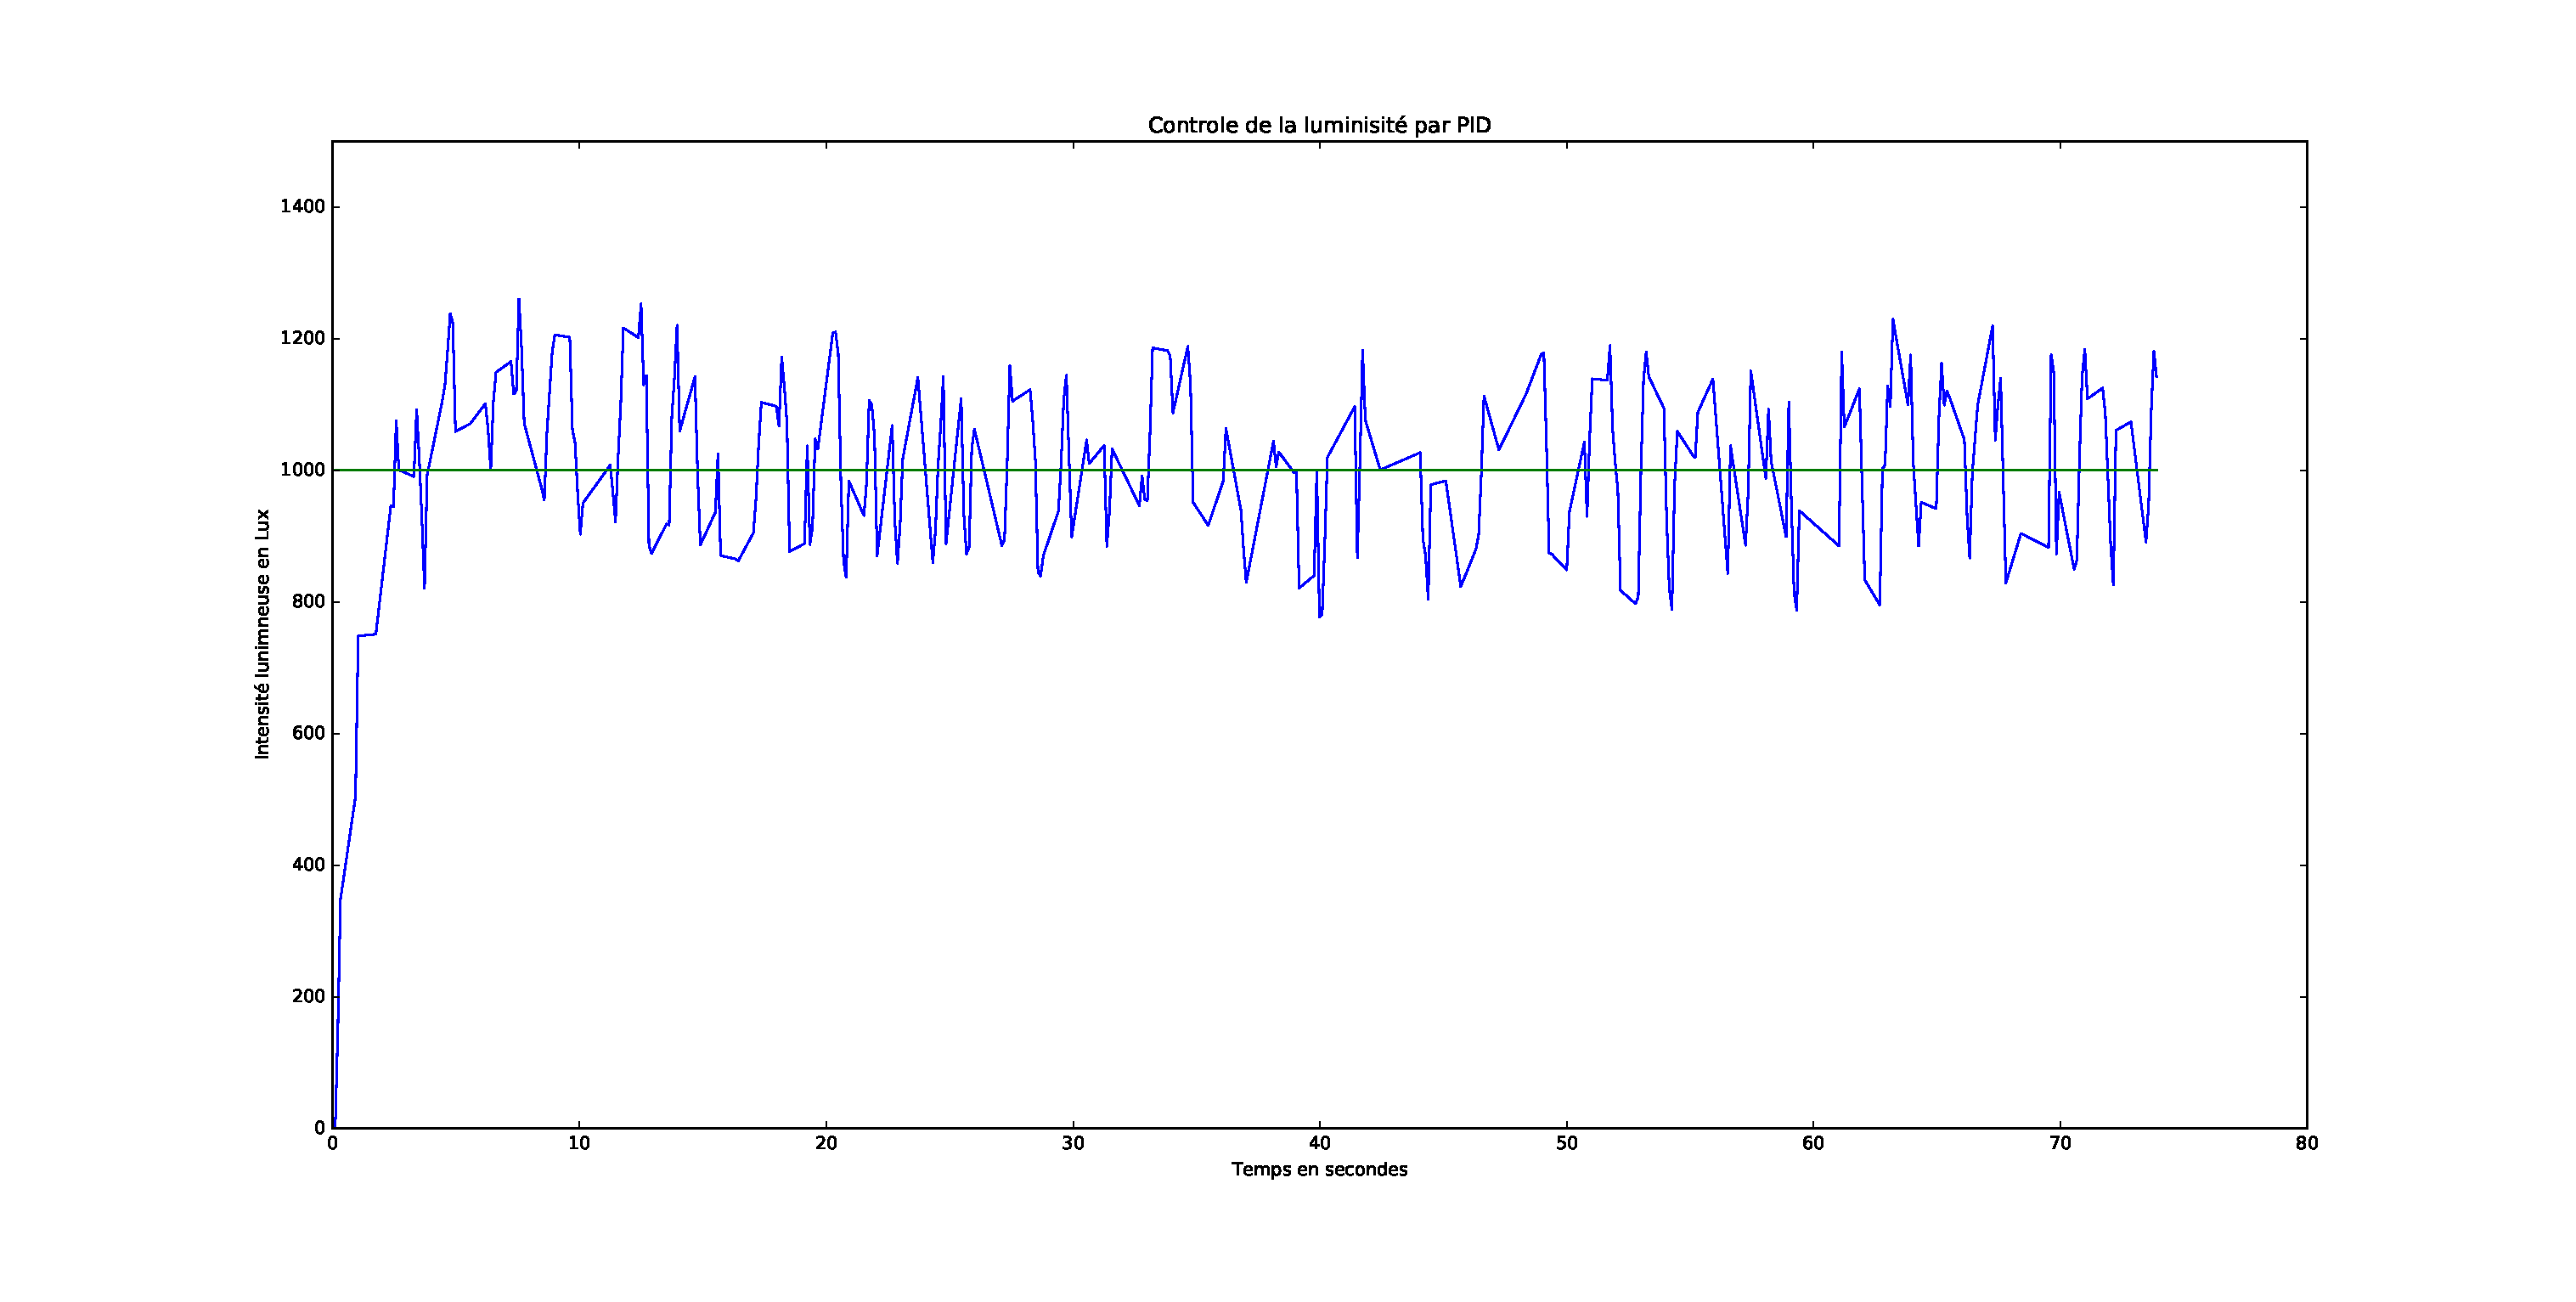
\includegraphics[scale=0.35]{PID.eps}
   \caption{\label{fig:pid} Contrôle de la luminosité par PID}
\end{figure}
Perfect


\section{Comapraison Methode de tuning}
\begin{table}[h]
    \begin{center}
        \begin{tabular}{r l}
            Manuelle & 25107.027529\\
            Ziegler Nichols & 39108.362240\\
            Génétique & 22262.563821
        \end{tabular}
    \end{center}
    \caption{Score de différentes méthodes de tuning de PID (moyenne sur 5 simulations)}
\end{table}

\subsection{Manuelle}
\begin{figure}[hb!]
   \centering
   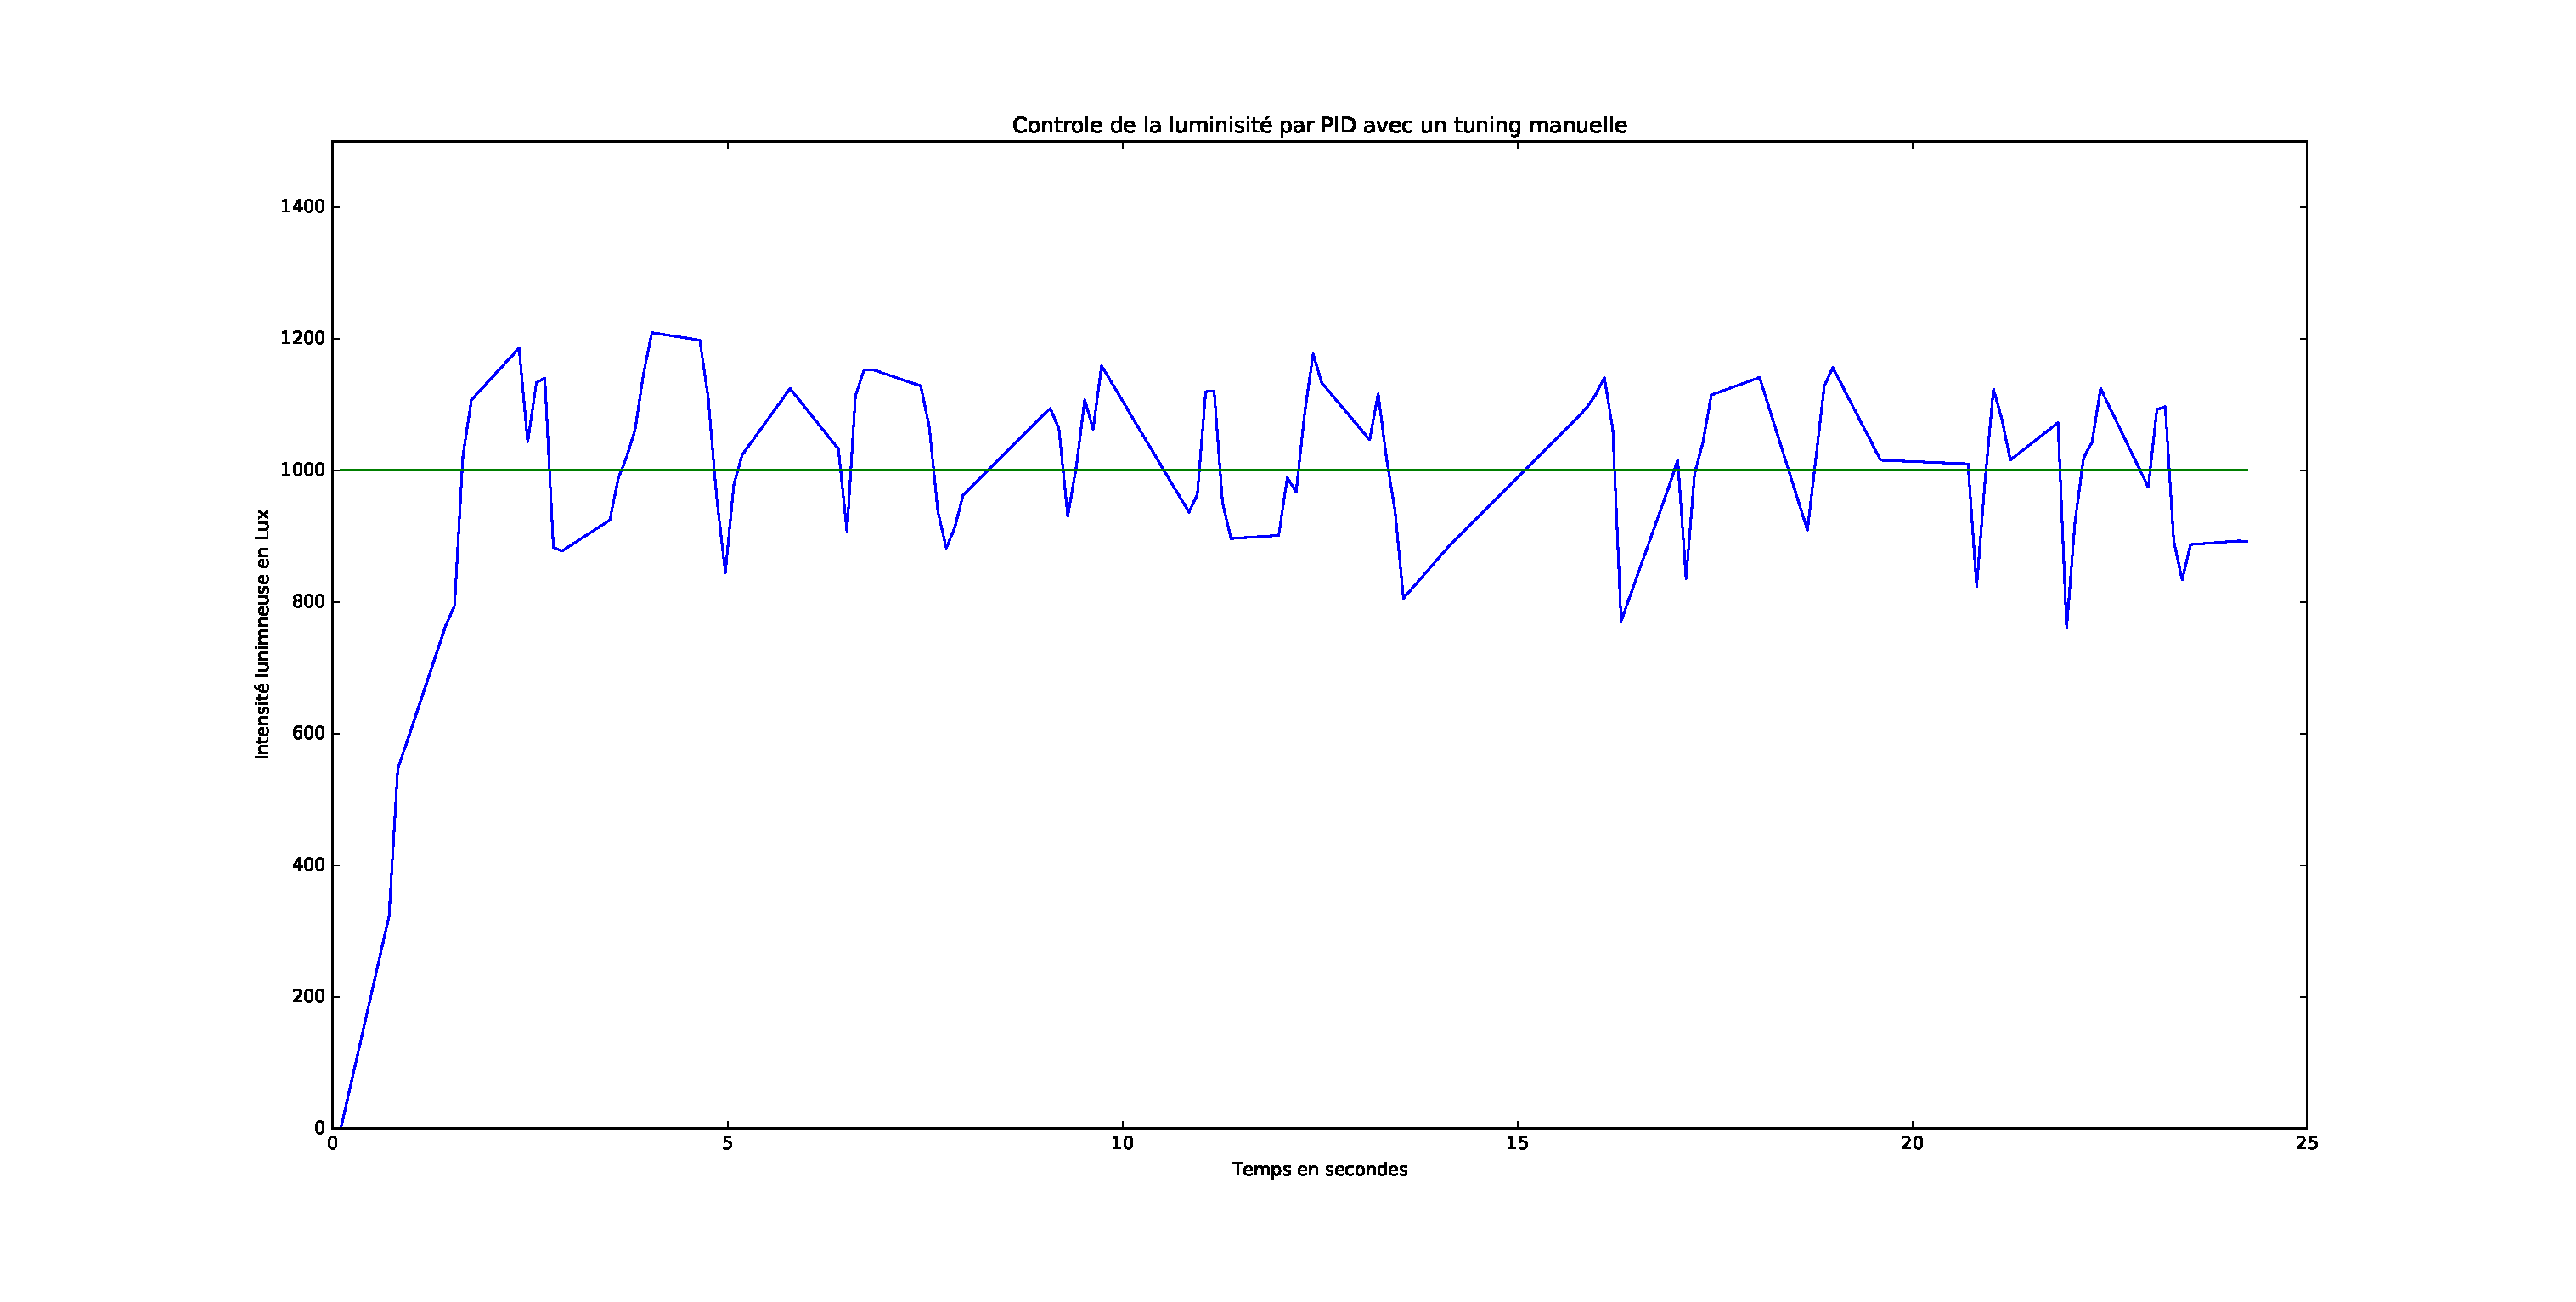
\includegraphics[scale=0.35]{Manuelle.eps}
   \caption{\label{fig:manuelle} Contrôle de la luminosité avec PID tunné à la main}
\end{figure}

\subsection{Ziegler Nichols}
\begin{figure}[hb!]
   \centering
   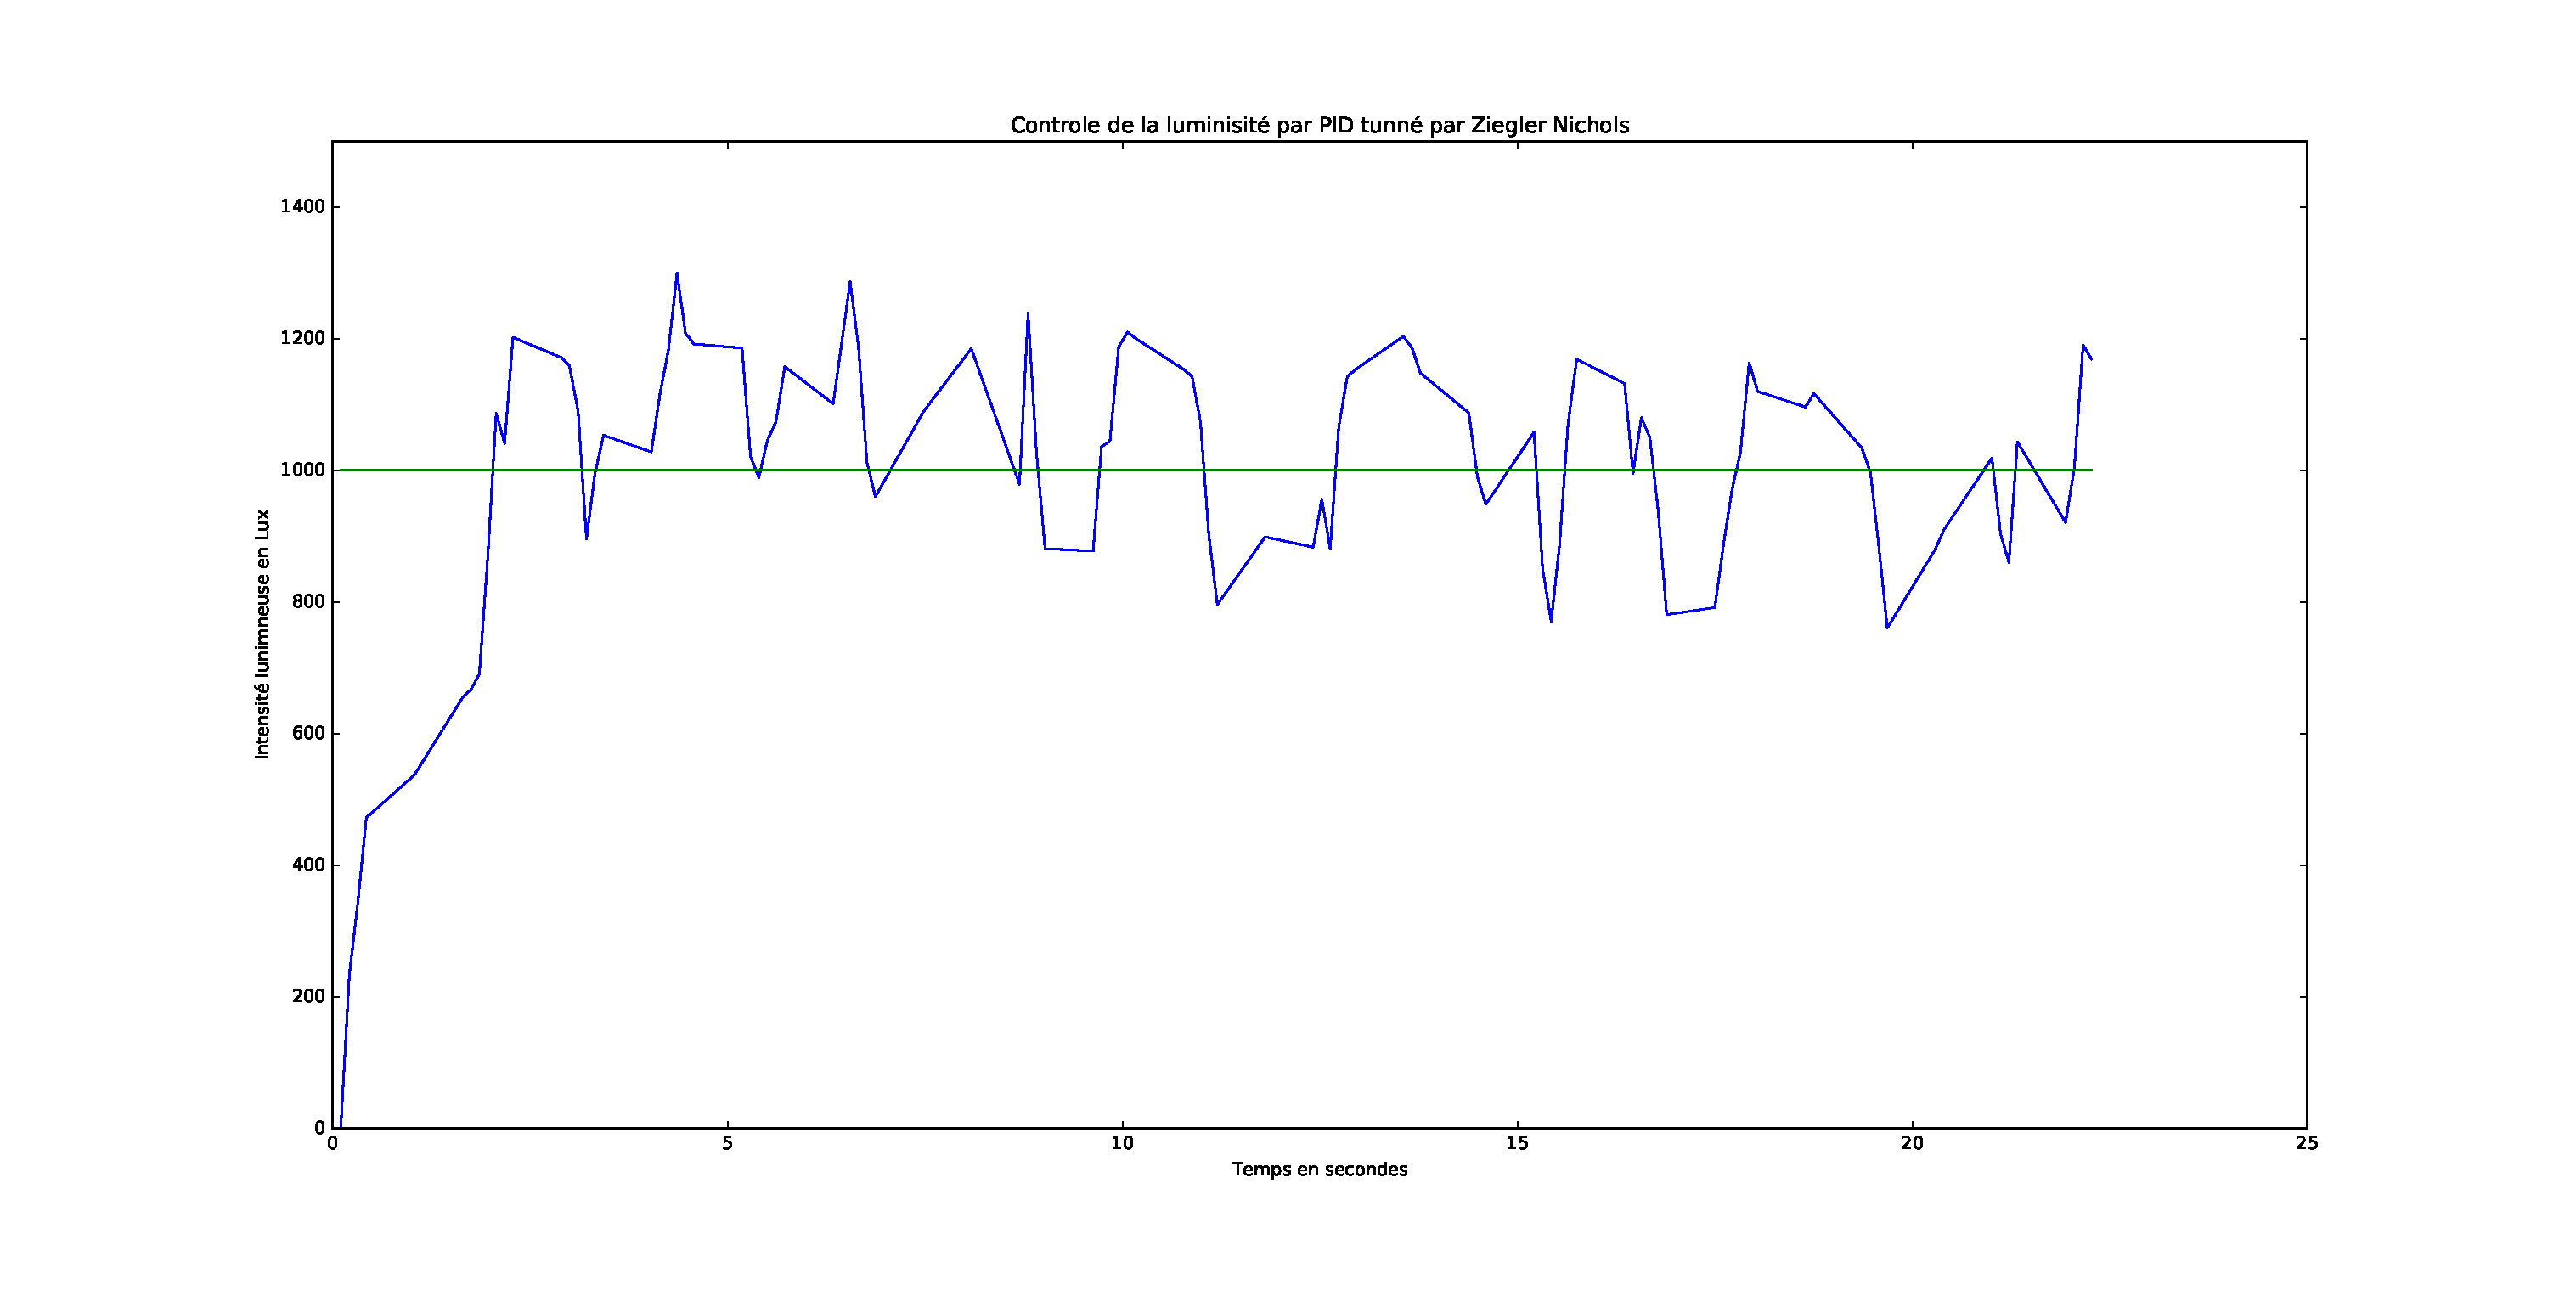
\includegraphics[scale=0.35]{Ziegler.eps}
   \caption{\label{fig:ziegler} Contrôle de la luminosité avec PID tunné avec Ziegler Nichols}
\end{figure}

\subsection{Génétique}
\begin{figure}[hb!]
   \centering
   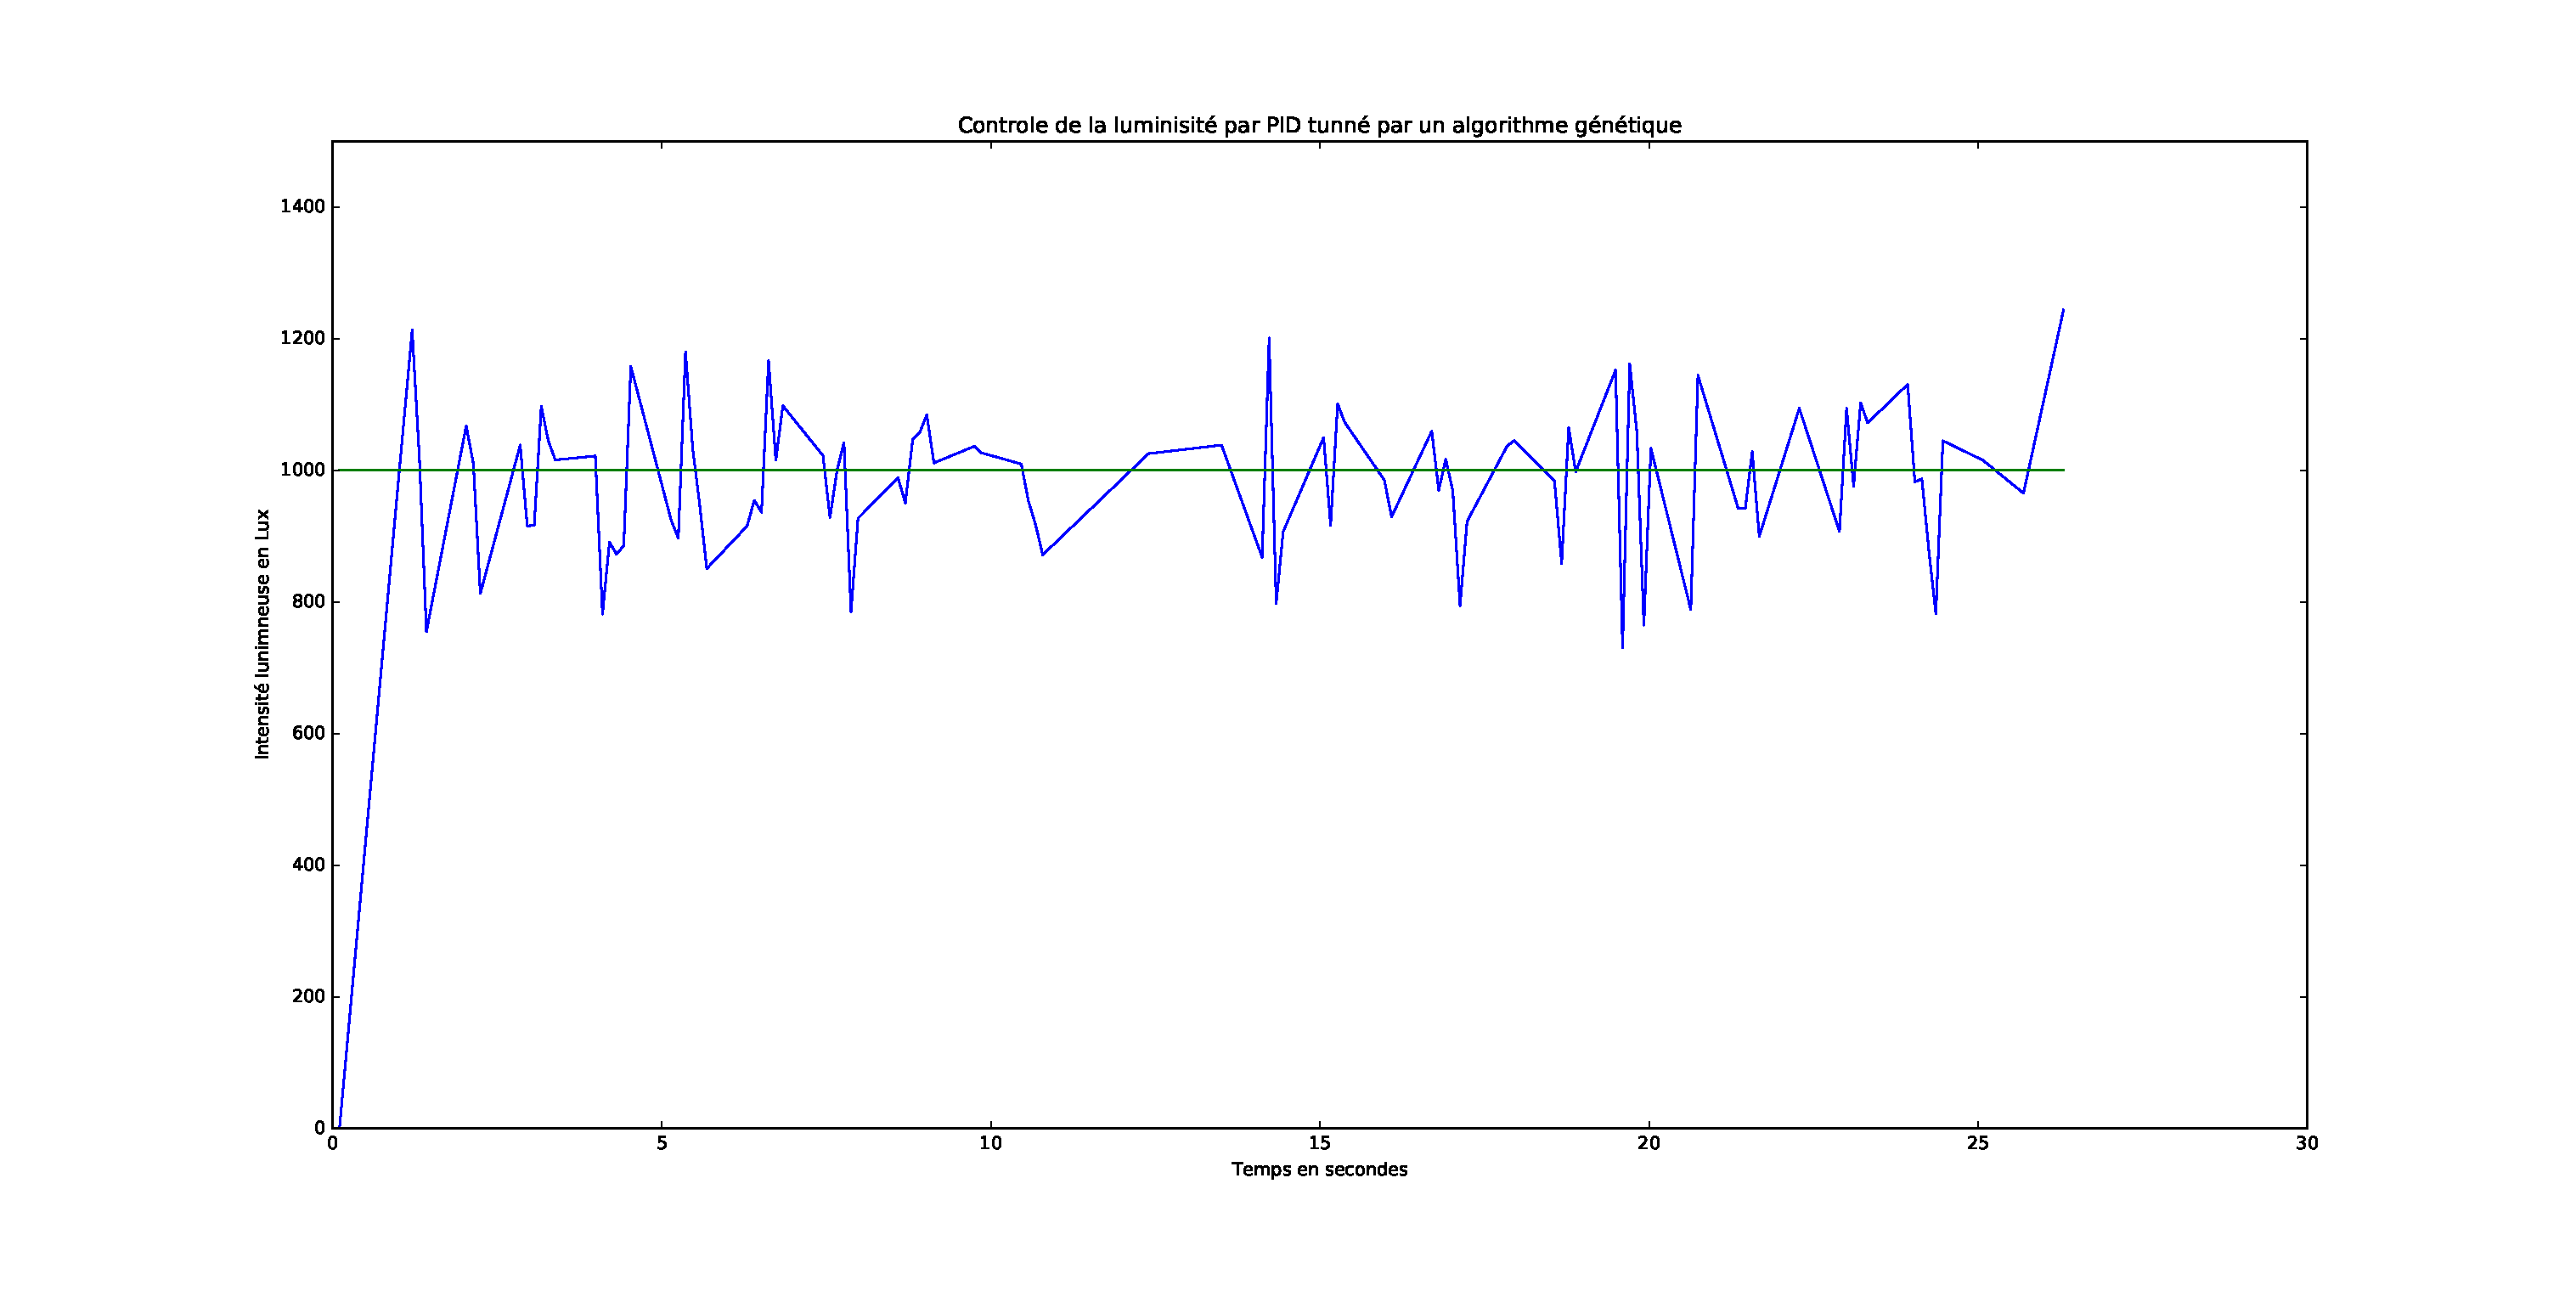
\includegraphics[scale=0.35]{Genetic.eps}
   \caption{\label{fig:genetique} Contrôle de la luminosité avec PID tunné avec un algorithme génétique}
\end{figure}

Nous avons fait tourné notre algorithme génétique sur 14 générations avec 50 chromosomes par génération.
\begin{figure}[hb!]
   \centering
   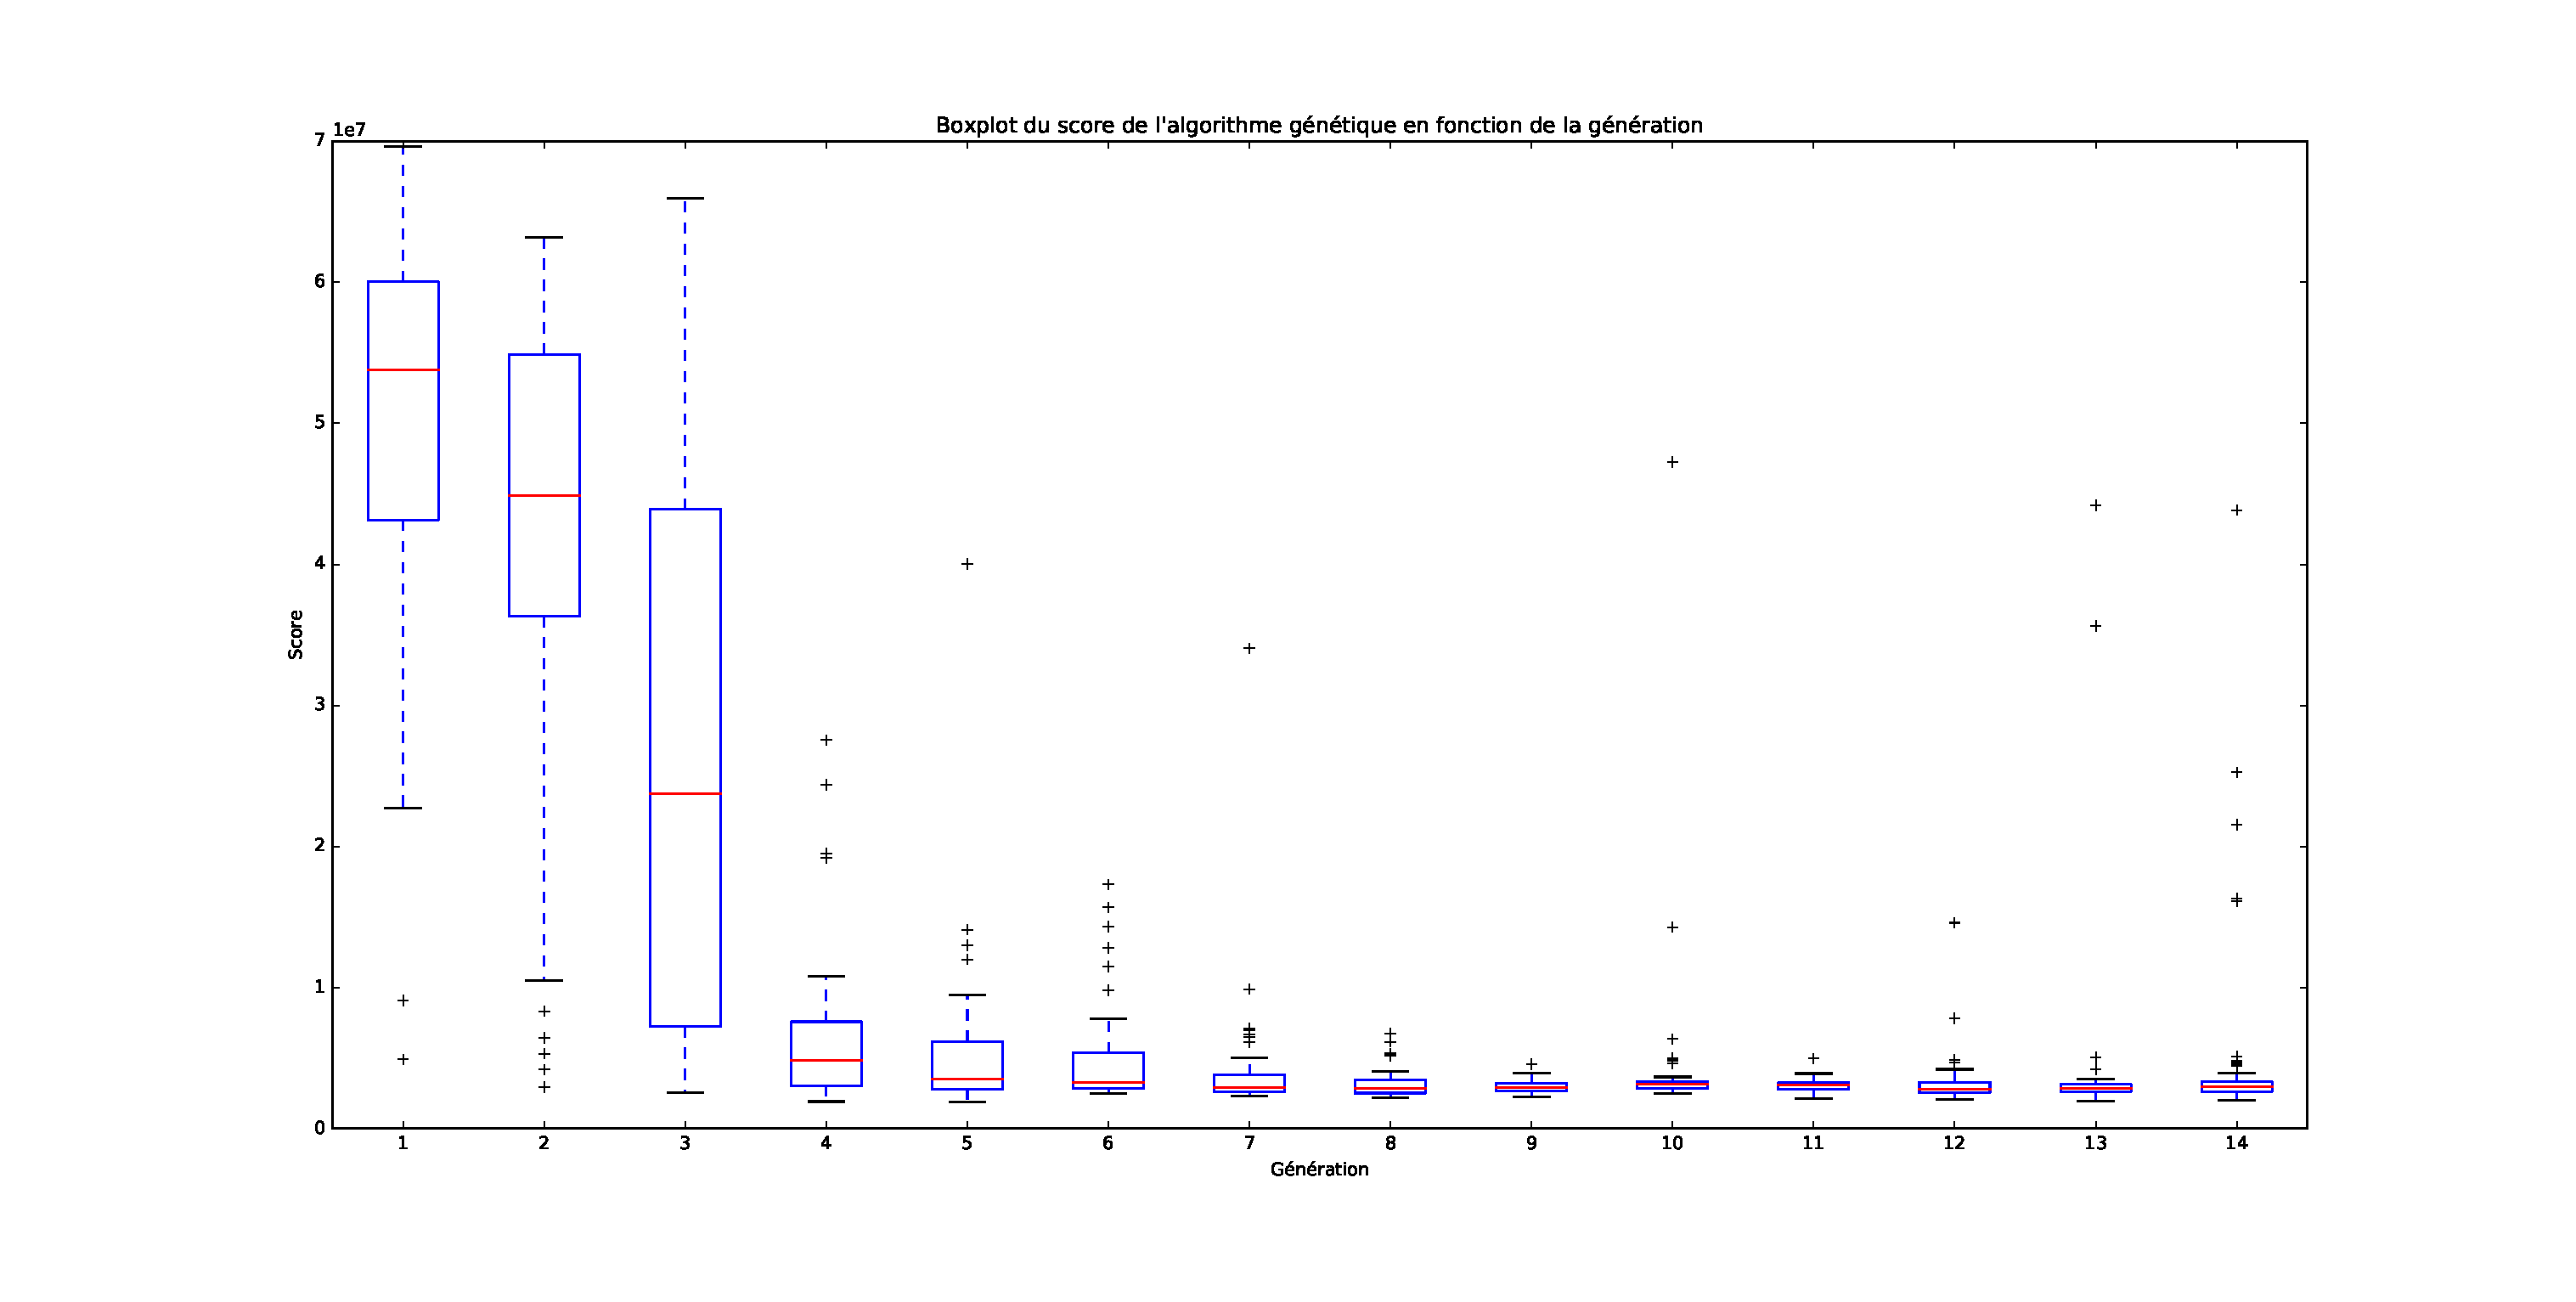
\includegraphics[scale=0.35]{GeneticBoxplot.eps}
    \caption{\label{fig:convergence} Convergence de l'algorithme génétique au cours des génération.}
\end{figure}

Nous pouvons voir une convergence du score assez rapide dans notre cas pour la détermination des kp kd ki.



\chapter{Discussion}
5.l’explication/discussion de ces résultats

\section{Application en situation réelle}

% TODO: Refactor les phrases, c'est vraiment juste du dump d'idées

Lors du Printemps des Sciences de l'Université Libre de Bruxelles, deux dispositifs pédagogiques ont été crées pour expliquer le projet aux visiteurs:

\begin{itemize}
\item Une petite serre avec des plantes, dans laquelle la température, la luminosité et l'humidité (air et sol) étaient mesurées en temps réel.
\item Une boite en plastique, modifiée pour accommoder un capteur de température, des ventilateurs et un sèche cheveux.
\end{itemize}

Dans la serre, l'algorithme PID était appliqué, tandis que dans la boite en plastique il s'agissait de Bang Bang. Les visiteurs pouvaient voir les données mesurées sur un écran, et donc voir en temps réel lorsque le système subissait une perturbation (et la correction qui était appliquée).

\section{Analyse des résultats}

\chapter{Conclusion et perspectives}

La mise en situation réelle lors du Printemps des Sciences nous a permis de tester nos algorithmes et résultats. La serre était suffisamment réactive lors des perturbations simulées pendant les démonstrations faites aux visiteurs, et la correction était faite de façon rapide et efficace. 

Il aurait été possible d'améliorer génétique % voir tirade d'Anthony qui avait l'air super scientifique mais qu'il veut pas me répéter.


\bibliographystyle{apalike}

\bibliography{biblio}
\addcontentsline{toc}{chapter}{Bibliographie}

\end{document}
